\documentclass[12pt,]{article}
\usepackage{lmodern}
\usepackage{amssymb,amsmath}
\usepackage{ifxetex,ifluatex}
\usepackage{fixltx2e} % provides \textsubscript
\ifnum 0\ifxetex 1\fi\ifluatex 1\fi=0 % if pdftex
  \usepackage[T1]{fontenc}
  \usepackage[utf8]{inputenc}
\else % if luatex or xelatex
  \ifxetex
    \usepackage{mathspec}
  \else
    \usepackage{fontspec}
  \fi
  \defaultfontfeatures{Ligatures=TeX,Scale=MatchLowercase}
\fi
% use upquote if available, for straight quotes in verbatim environments
\IfFileExists{upquote.sty}{\usepackage{upquote}}{}
% use microtype if available
\IfFileExists{microtype.sty}{%
\usepackage{microtype}
\UseMicrotypeSet[protrusion]{basicmath} % disable protrusion for tt fonts
}{}
\usepackage[margin=2.54cm]{geometry}
\usepackage{hyperref}
\hypersetup{unicode=true,
            pdftitle={Are the Thermoclines on Wisconsin Lakes Moving Deeper?},
            pdfauthor={Keith Bollt},
            pdfborder={0 0 0},
            breaklinks=true}
\urlstyle{same}  % don't use monospace font for urls
\usepackage{color}
\usepackage{fancyvrb}
\newcommand{\VerbBar}{|}
\newcommand{\VERB}{\Verb[commandchars=\\\{\}]}
\DefineVerbatimEnvironment{Highlighting}{Verbatim}{commandchars=\\\{\}}
% Add ',fontsize=\small' for more characters per line
\usepackage{framed}
\definecolor{shadecolor}{RGB}{248,248,248}
\newenvironment{Shaded}{\begin{snugshade}}{\end{snugshade}}
\newcommand{\KeywordTok}[1]{\textcolor[rgb]{0.13,0.29,0.53}{\textbf{#1}}}
\newcommand{\DataTypeTok}[1]{\textcolor[rgb]{0.13,0.29,0.53}{#1}}
\newcommand{\DecValTok}[1]{\textcolor[rgb]{0.00,0.00,0.81}{#1}}
\newcommand{\BaseNTok}[1]{\textcolor[rgb]{0.00,0.00,0.81}{#1}}
\newcommand{\FloatTok}[1]{\textcolor[rgb]{0.00,0.00,0.81}{#1}}
\newcommand{\ConstantTok}[1]{\textcolor[rgb]{0.00,0.00,0.00}{#1}}
\newcommand{\CharTok}[1]{\textcolor[rgb]{0.31,0.60,0.02}{#1}}
\newcommand{\SpecialCharTok}[1]{\textcolor[rgb]{0.00,0.00,0.00}{#1}}
\newcommand{\StringTok}[1]{\textcolor[rgb]{0.31,0.60,0.02}{#1}}
\newcommand{\VerbatimStringTok}[1]{\textcolor[rgb]{0.31,0.60,0.02}{#1}}
\newcommand{\SpecialStringTok}[1]{\textcolor[rgb]{0.31,0.60,0.02}{#1}}
\newcommand{\ImportTok}[1]{#1}
\newcommand{\CommentTok}[1]{\textcolor[rgb]{0.56,0.35,0.01}{\textit{#1}}}
\newcommand{\DocumentationTok}[1]{\textcolor[rgb]{0.56,0.35,0.01}{\textbf{\textit{#1}}}}
\newcommand{\AnnotationTok}[1]{\textcolor[rgb]{0.56,0.35,0.01}{\textbf{\textit{#1}}}}
\newcommand{\CommentVarTok}[1]{\textcolor[rgb]{0.56,0.35,0.01}{\textbf{\textit{#1}}}}
\newcommand{\OtherTok}[1]{\textcolor[rgb]{0.56,0.35,0.01}{#1}}
\newcommand{\FunctionTok}[1]{\textcolor[rgb]{0.00,0.00,0.00}{#1}}
\newcommand{\VariableTok}[1]{\textcolor[rgb]{0.00,0.00,0.00}{#1}}
\newcommand{\ControlFlowTok}[1]{\textcolor[rgb]{0.13,0.29,0.53}{\textbf{#1}}}
\newcommand{\OperatorTok}[1]{\textcolor[rgb]{0.81,0.36,0.00}{\textbf{#1}}}
\newcommand{\BuiltInTok}[1]{#1}
\newcommand{\ExtensionTok}[1]{#1}
\newcommand{\PreprocessorTok}[1]{\textcolor[rgb]{0.56,0.35,0.01}{\textit{#1}}}
\newcommand{\AttributeTok}[1]{\textcolor[rgb]{0.77,0.63,0.00}{#1}}
\newcommand{\RegionMarkerTok}[1]{#1}
\newcommand{\InformationTok}[1]{\textcolor[rgb]{0.56,0.35,0.01}{\textbf{\textit{#1}}}}
\newcommand{\WarningTok}[1]{\textcolor[rgb]{0.56,0.35,0.01}{\textbf{\textit{#1}}}}
\newcommand{\AlertTok}[1]{\textcolor[rgb]{0.94,0.16,0.16}{#1}}
\newcommand{\ErrorTok}[1]{\textcolor[rgb]{0.64,0.00,0.00}{\textbf{#1}}}
\newcommand{\NormalTok}[1]{#1}
\usepackage{longtable,booktabs}
\usepackage{graphicx,grffile}
\makeatletter
\def\maxwidth{\ifdim\Gin@nat@width>\linewidth\linewidth\else\Gin@nat@width\fi}
\def\maxheight{\ifdim\Gin@nat@height>\textheight\textheight\else\Gin@nat@height\fi}
\makeatother
% Scale images if necessary, so that they will not overflow the page
% margins by default, and it is still possible to overwrite the defaults
% using explicit options in \includegraphics[width, height, ...]{}
\setkeys{Gin}{width=\maxwidth,height=\maxheight,keepaspectratio}
\IfFileExists{parskip.sty}{%
\usepackage{parskip}
}{% else
\setlength{\parindent}{0pt}
\setlength{\parskip}{6pt plus 2pt minus 1pt}
}
\setlength{\emergencystretch}{3em}  % prevent overfull lines
\providecommand{\tightlist}{%
  \setlength{\itemsep}{0pt}\setlength{\parskip}{0pt}}
\setcounter{secnumdepth}{5}
% Redefines (sub)paragraphs to behave more like sections
\ifx\paragraph\undefined\else
\let\oldparagraph\paragraph
\renewcommand{\paragraph}[1]{\oldparagraph{#1}\mbox{}}
\fi
\ifx\subparagraph\undefined\else
\let\oldsubparagraph\subparagraph
\renewcommand{\subparagraph}[1]{\oldsubparagraph{#1}\mbox{}}
\fi

%%% Use protect on footnotes to avoid problems with footnotes in titles
\let\rmarkdownfootnote\footnote%
\def\footnote{\protect\rmarkdownfootnote}

%%% Change title format to be more compact
\usepackage{titling}

% Create subtitle command for use in maketitle
\newcommand{\subtitle}[1]{
  \posttitle{
    \begin{center}\large#1\end{center}
    }
}

\setlength{\droptitle}{-2em}

  \title{Are the Thermoclines on Wisconsin Lakes Moving Deeper?}
    \pretitle{\vspace{\droptitle}\centering\huge}
  \posttitle{\par}
  \subtitle{Web address for GitHub repository}
  \author{Keith Bollt}
    \preauthor{\centering\large\emph}
  \postauthor{\par}
    \date{}
    \predate{}\postdate{}
  

\begin{document}
\maketitle
\begin{abstract}
For this project, I was interested in determining if thermoclines in
five Wisconsin lakes are trending deeper over time, possibly due to
climate change. I looked at physical and chemical data from the NTLR
dataset, specifically temperature and dissolved oxygen levels at 7
meters depth between June 20 and September 21 from every year data was
available between 1984 and 2016. Initial data visualization did not
promise significant trends that would point to climate change. I ran
four total tests on the dataset: a repeated measures ANOVA on the
combined dataset for both variables, and a seasonal Mann Kendall on each
of the five lakes for both variables. I found that there was not a
significant trend in temperature or oxygen on the five lakes as a whole,
and that no individual lake exhibited both a significant increase in
temperature and a significant decrease in dissolved oxygen at 7 meters
depth. In my conclusion, I discuss that for incremental climate change,
the thermocline may not move because it is a result of a lake's relative
physical conditions. Further tests would likely reveal that the
thermocline is steeper.
\end{abstract}

\begin{Shaded}
\begin{Highlighting}[]
\CommentTok{#Setting up session and loading all packages I think I might need}
\KeywordTok{getwd}\NormalTok{()}
\end{Highlighting}
\end{Shaded}

\begin{verbatim}
## [1] "V:/ENV872BadgerThermoclines"
\end{verbatim}

\begin{Shaded}
\begin{Highlighting}[]
\KeywordTok{library}\NormalTok{(tidyverse)}
\end{Highlighting}
\end{Shaded}

\begin{verbatim}
## Warning: package 'tidyverse' was built under R version 3.5.2
\end{verbatim}

\begin{verbatim}
## -- Attaching packages --------------------------------------------------------------------------------- tidyverse 1.2.1 --
\end{verbatim}

\begin{verbatim}
## v ggplot2 3.1.0     v purrr   0.2.5
## v tibble  1.4.2     v dplyr   0.7.8
## v tidyr   0.8.2     v stringr 1.3.1
## v readr   1.3.1     v forcats 0.3.0
\end{verbatim}

\begin{verbatim}
## Warning: package 'ggplot2' was built under R version 3.5.2
\end{verbatim}

\begin{verbatim}
## Warning: package 'tibble' was built under R version 3.5.2
\end{verbatim}

\begin{verbatim}
## Warning: package 'tidyr' was built under R version 3.5.2
\end{verbatim}

\begin{verbatim}
## Warning: package 'readr' was built under R version 3.5.2
\end{verbatim}

\begin{verbatim}
## Warning: package 'purrr' was built under R version 3.5.2
\end{verbatim}

\begin{verbatim}
## Warning: package 'dplyr' was built under R version 3.5.2
\end{verbatim}

\begin{verbatim}
## Warning: package 'stringr' was built under R version 3.5.2
\end{verbatim}

\begin{verbatim}
## Warning: package 'forcats' was built under R version 3.5.2
\end{verbatim}

\begin{verbatim}
## -- Conflicts ------------------------------------------------------------------------------------ tidyverse_conflicts() --
## x dplyr::filter() masks stats::filter()
## x dplyr::lag()    masks stats::lag()
\end{verbatim}

\begin{Shaded}
\begin{Highlighting}[]
\KeywordTok{library}\NormalTok{(lubridate)}
\end{Highlighting}
\end{Shaded}

\begin{verbatim}
## Warning: package 'lubridate' was built under R version 3.5.2
\end{verbatim}

\begin{verbatim}
## 
## Attaching package: 'lubridate'
\end{verbatim}

\begin{verbatim}
## The following object is masked from 'package:base':
## 
##     date
\end{verbatim}

\begin{Shaded}
\begin{Highlighting}[]
\KeywordTok{library}\NormalTok{(ggplot2)}
\KeywordTok{library}\NormalTok{(multcompView)}
\end{Highlighting}
\end{Shaded}

\begin{verbatim}
## Warning: package 'multcompView' was built under R version 3.5.2
\end{verbatim}

\begin{Shaded}
\begin{Highlighting}[]
\KeywordTok{library}\NormalTok{(nlme)}
\end{Highlighting}
\end{Shaded}

\begin{verbatim}
## 
## Attaching package: 'nlme'
\end{verbatim}

\begin{verbatim}
## The following object is masked from 'package:dplyr':
## 
##     collapse
\end{verbatim}

\begin{Shaded}
\begin{Highlighting}[]
\KeywordTok{library}\NormalTok{(lsmeans)}
\end{Highlighting}
\end{Shaded}

\begin{verbatim}
## Warning: package 'lsmeans' was built under R version 3.5.2
\end{verbatim}

\begin{verbatim}
## Loading required package: emmeans
\end{verbatim}

\begin{verbatim}
## Warning: package 'emmeans' was built under R version 3.5.2
\end{verbatim}

\begin{verbatim}
## The 'lsmeans' package is now basically a front end for 'emmeans'.
## Users are encouraged to switch the rest of the way.
## See help('transition') for more information, including how to
## convert old 'lsmeans' objects and scripts to work with 'emmeans'.
\end{verbatim}

\begin{Shaded}
\begin{Highlighting}[]
\CommentTok{#install.packages("trend")}
\KeywordTok{library}\NormalTok{(trend)}
\end{Highlighting}
\end{Shaded}

\begin{verbatim}
## Warning: package 'trend' was built under R version 3.5.3
\end{verbatim}

\begin{Shaded}
\begin{Highlighting}[]
\CommentTok{#setting a theme for plots}
\NormalTok{mytheme <-}\StringTok{ }\KeywordTok{theme_classic}\NormalTok{(}\DataTypeTok{base_size =} \FloatTok{12.2696}\NormalTok{)}\OperatorTok{+}
\StringTok{  }\KeywordTok{theme}\NormalTok{(}\DataTypeTok{axis.text =} \KeywordTok{element_text}\NormalTok{(}\DataTypeTok{color =} \StringTok{"Blue"}\NormalTok{),}
  \DataTypeTok{legend.position =} \StringTok{"top"}\NormalTok{)}
\NormalTok{  plot.title =}\StringTok{ }\KeywordTok{element_text}\NormalTok{(}\DataTypeTok{hjust =} \FloatTok{0.5}\NormalTok{)}
\KeywordTok{theme_set}\NormalTok{(mytheme)}
\end{Highlighting}
\end{Shaded}

\begin{Shaded}
\begin{Highlighting}[]
\CommentTok{#Reading in the raw lake dataset}
\NormalTok{NTLR_raw <-}\StringTok{ }\KeywordTok{read.csv}\NormalTok{(}\StringTok{"V:/ENV_872_Project_Directory/Data/Raw/NTL-LTER_Lake_ChemistryPhysics_Raw.csv"}\NormalTok{)}
\KeywordTok{View}\NormalTok{(NTLR_raw)}

\CommentTok{#Changing the date column to read as a date}
\KeywordTok{class}\NormalTok{(NTLR_raw}\OperatorTok{$}\NormalTok{sampledate)}
\end{Highlighting}
\end{Shaded}

\begin{verbatim}
## [1] "factor"
\end{verbatim}

\begin{Shaded}
\begin{Highlighting}[]
\NormalTok{NTLR_raw}\OperatorTok{$}\NormalTok{sampledate <-}\StringTok{ }\KeywordTok{as.Date}\NormalTok{(NTLR_raw}\OperatorTok{$}\NormalTok{sampledate, }\DataTypeTok{format=}\StringTok{"%m/%d/%y"}\NormalTok{)}
\KeywordTok{class}\NormalTok{(NTLR_raw}\OperatorTok{$}\NormalTok{sampledate)}
\end{Highlighting}
\end{Shaded}

\begin{verbatim}
## [1] "Date"
\end{verbatim}

Research Question and Rationale: The crux of this project is to
determine if the thermoclines on each of the 9 Wisconsin lakes in the
NTL-LTER chemistry and physics dataset have moved over the course of the
33 years of data between 1984 and 2016. I am interested in this question
because as a flyfisherman, I have an interest in coldwater fisheries
that rely on thermoclines to survive the summer weather. Perhaps climate
change is affecting where the thermocline sets up, and therefore
shrinking the available summer habitat of trout.

In order to determine whether thermoclines on these lakes are moving
deeper in the water column, I need to set a benchmark definition for a
thermocline. It looks like there is not enough temporal resolution to
measure close-to-continuous change in thermocline depth over the course
of a given season. Likewise, there is not enough close-to-continous
depth measurements taken at each lake, nor is there consistant data
taken below 10 meters of depth. As such, I will compare what is
occurring at a constant depth near the expected thermocline location at
each lake over time. The depth that I chose for the purpose of this
study is 7 meters. 7 meters, I know from my experience as a fisherman,
is on the shallow end of where a thermocline sets up in a northern US
lake. In addition, there is enough temporal resolution at seven meters
to perform statistical analysis on five of the lakes in the raw dataset.
Therefore, evaluating what is happening at 7m depth in each lake will
give a good idea what sorts of conditions trout are dealing with in
these lakes in the summmer. I know from data visualization that did not
make my final report that there is much more variation by year at 7
meters depth than at, say, 10 meters depth. This indicates that 7 meters
is indeed a pretty good estimation of thermocline location for these
lakes. Looking for change at 7 meters should give me a good picture of
whether the thermocline in these lakes is changing over time.

I will look at two indicators of thermocline establishment at 7 meters:
temperature and dissolved oxygen content. I would expect water at or
below the thermocline to have low temperatures and hypoxic conditions
(low oxygen levels). If the thermoclines on these lakes are trending
deeper over the course of my dataset, I would expect most of the lakes
to show increasing temperatures and increasing dissolved oxygen levels
at a 7 meter depth.

My research question, then, is as follows:

How have temperature and oxygen conditions changed at 7 meters depth in
a series of Wisconsin Lakes? Is climate change affecting where the
thermocline sets up in these lakes?

Dataset Information:

The dataset used for this project was prepared for Environmental Data
Analytics (ENV 872L) at Duke University's Nicholas School of the
Environment for the spring 2019 semester by Professor Kateri Salk.The
dataset contains physical and chemical data from nine lakes in
Wisconsin. The data was collected between 1984 and 2016 as part of the
NSF-funded North Temperate Lakes Long Term Ecological Research Station.
The data is measured at a station in the middle of each of the nine
lakes. Generally, the data was collected in the morning. The data is
taken at increments, and most data is taken at or below ten meters
depth. The temporal resolution varies across lakes. Some lakes only have
a few years of data, while others have ample data from most or all
years.Data was collected at irregular 1 to 7 day increments from May
through August of each year. The data was taken during periods of no ice
on the lake. This means that there is little data during the winter
months. While there are several different measurements taken at these
lakes, the two variables that the thermocline study focuses on are
dissolved oxygen and temperature. A table summarizing the data structure
of this project is provided at the end of this section. Data collection
techniques used during the period 1984-1990 were described by Carpenter
and Kitchell (1993) and data collection techniques for 1991-1997 were
described by Carpenter et al. (2001).

Carpenter, S.R. and J.F. Kitchell (eds.). 1993. The Trophic Cascade in
Lakes. Cambridge University Press, Cambridge, England.

Carpenter, S.R., J.J. Cole, J.R. Hodgson, J.F. Kitchell, M.L. Pace,D.
Bade, K.L. Cottingham, T.E. Essington, J.N. Houser and D.E. Schindler.
2001. Trophic cascades, nutrients and lake productivity: whole-lake
experiments. Ecological Monographs 71: 163-186."

Table Summarizing Project Data Structure:

\begin{longtable}[]{@{}ll@{}}
\toprule
\begin{minipage}[b]{0.33\columnwidth}\raggedright\strut
Element\strut
\end{minipage} & \begin{minipage}[b]{0.61\columnwidth}\raggedright\strut
Details\strut
\end{minipage}\tabularnewline
\midrule
\endhead
\begin{minipage}[t]{0.33\columnwidth}\raggedright\strut
Data Source\strut
\end{minipage} & \begin{minipage}[t]{0.61\columnwidth}\raggedright\strut
North Temperate Lakes Long Term Ecological Research Station\strut
\end{minipage}\tabularnewline
\begin{minipage}[t]{0.33\columnwidth}\raggedright\strut
Data Scraper\strut
\end{minipage} & \begin{minipage}[t]{0.61\columnwidth}\raggedright\strut
Professor Kateri Salk, PhD, Duke University;
\href{mailto:kateri.salk@duke.edu}{\nolinkurl{kateri.salk@duke.edu}}\strut
\end{minipage}\tabularnewline
\begin{minipage}[t]{0.33\columnwidth}\raggedright\strut
More Information about Data\strut
\end{minipage} & \begin{minipage}[t]{0.61\columnwidth}\raggedright\strut
\url{https://lter.limnology.wisc.edu/about/overview}\strut
\end{minipage}\tabularnewline
\begin{minipage}[t]{0.33\columnwidth}\raggedright\strut
Link to Access Data\strut
\end{minipage} & \begin{minipage}[t]{0.61\columnwidth}\raggedright\strut
\url{https://lter.limnology.wisc.edu/data}\strut
\end{minipage}\tabularnewline
\begin{minipage}[t]{0.33\columnwidth}\raggedright\strut
Dimensions of Raw Dataset\strut
\end{minipage} & \begin{minipage}[t]{0.61\columnwidth}\raggedright\strut
38,614 Observations of 11 variables over nine lakes\strut
\end{minipage}\tabularnewline
\begin{minipage}[t]{0.33\columnwidth}\raggedright\strut
Dimensions of Processed Dataset\strut
\end{minipage} & \begin{minipage}[t]{0.61\columnwidth}\raggedright\strut
1,116 Observations of 8 variables over five lakes\strut
\end{minipage}\tabularnewline
\begin{minipage}[t]{0.33\columnwidth}\raggedright\strut
Variables in Processed Dataset\strut
\end{minipage} & \begin{minipage}[t]{0.61\columnwidth}\raggedright\strut
lakename (lake name), year4 (year), daynum (Julian day number),
sampledate (date of observation), depth of observation (in meters),
temperature\_C (lake temperature in degrees Celsius), dissolved Oxygen
(percent dissolved Oxygen), Week (numbered week of the year)\strut
\end{minipage}\tabularnewline
\begin{minipage}[t]{0.33\columnwidth}\raggedright\strut
Temporal Resolution of Processed Dataset\strut
\end{minipage} & \begin{minipage}[t]{0.61\columnwidth}\raggedright\strut
Irregular collection intervals from June 20 to September 21,
1984-2016\strut
\end{minipage}\tabularnewline
\bottomrule
\end{longtable}

Exploratory Data Analysis Wrangling:

In order to answer my research question, I need to wrangle my data to
only include the data relevant to my study and to organize it by lake. I
only want data during the summer months (June 20 through September 21)
because this is the time of year when the thermocline is the steepest
and coldwater fish are the most thermally stressed. I also only want
data collected at a 7 meter depth. My first step is to filter my raw
data to generate a dataset for each of the nine lakes.This data summary
gives me the names of the nine lakes.

\begin{Shaded}
\begin{Highlighting}[]
\KeywordTok{unique}\NormalTok{(NTLR_raw}\OperatorTok{$}\NormalTok{lakename)  }
\end{Highlighting}
\end{Shaded}

\begin{verbatim}
## [1] Paul Lake         Peter Lake        Tuesday Lake      East Long Lake   
## [5] West Long Lake    Central Long Lake Hummingbird Lake  Crampton Lake    
## [9] Ward Lake        
## 9 Levels: Central Long Lake Crampton Lake ... West Long Lake
\end{verbatim}

\begin{Shaded}
\begin{Highlighting}[]
\NormalTok{Paullake_raw <-}\StringTok{ }\NormalTok{NTLR_raw }\OperatorTok
\StringTok{  }\KeywordTok{filter}\NormalTok{(lakename }\OperatorTok{==}\StringTok{ "Paul Lake"}\NormalTok{)}
\end{Highlighting}
\end{Shaded}

\begin{verbatim}
## Warning: package 'bindrcpp' was built under R version 3.5.2
\end{verbatim}

\begin{Shaded}
\begin{Highlighting}[]
\NormalTok{Peterlake_raw <-}\StringTok{ }\NormalTok{NTLR_raw }\OperatorTok
\StringTok{  }\KeywordTok{filter}\NormalTok{(lakename }\OperatorTok{==}\StringTok{ "Peter Lake"}\NormalTok{)}
\NormalTok{Tuesdaylake_raw <-}\StringTok{ }\NormalTok{NTLR_raw }\OperatorTok
\StringTok{  }\KeywordTok{filter}\NormalTok{(lakename }\OperatorTok{==}\StringTok{ "Tuesday Lake"}\NormalTok{)}
\NormalTok{Eastlonglake_raw <-}\StringTok{ }\NormalTok{NTLR_raw }\OperatorTok
\StringTok{  }\KeywordTok{filter}\NormalTok{(lakename }\OperatorTok{==}\StringTok{ "East Long Lake"}\NormalTok{)}
\NormalTok{Westlonglake_raw <-}\StringTok{ }\NormalTok{NTLR_raw }\OperatorTok
\StringTok{  }\KeywordTok{filter}\NormalTok{(lakename }\OperatorTok{==}\StringTok{ "West Long Lake"}\NormalTok{)}
\NormalTok{Centrallonglake_raw <-}\StringTok{ }\NormalTok{NTLR_raw }\OperatorTok
\StringTok{  }\KeywordTok{filter}\NormalTok{(lakename }\OperatorTok{==}\StringTok{ "Central Long Lake"}\NormalTok{)}
\NormalTok{Hummingbirdlake_raw <-}\StringTok{ }\NormalTok{NTLR_raw }\OperatorTok
\StringTok{  }\KeywordTok{filter}\NormalTok{(lakename }\OperatorTok{==}\StringTok{ "Hummingbird Lake"}\NormalTok{)}
\NormalTok{Cramptonlake_raw <-}\StringTok{ }\NormalTok{NTLR_raw }\OperatorTok
\StringTok{  }\KeywordTok{filter}\NormalTok{(lakename }\OperatorTok{==}\StringTok{ "Crampton Lake"}\NormalTok{)}
\NormalTok{Wardlake_raw <-}\StringTok{ }\NormalTok{NTLR_raw }\OperatorTok
\StringTok{  }\KeywordTok{filter}\NormalTok{(lakename }\OperatorTok{==}\StringTok{ "Ward Lake"}\NormalTok{)}
\end{Highlighting}
\end{Shaded}

My next step is to filter my dataset to only include data collected at 7
meters depths between June 20 and September 21. I also checked the
dimensions of my wrangled data to make sure each lake still had enough
datapoints to perform statistical analysis on.

\begin{Shaded}
\begin{Highlighting}[]
\NormalTok{Paullake_processed <-}\StringTok{ }\NormalTok{Paullake_raw }\OperatorTok
\StringTok{  }\KeywordTok{filter}\NormalTok{(depth }\OperatorTok{==}\StringTok{ }\DecValTok{7}\NormalTok{, daynum }\OperatorTok\StringTok{ }\DecValTok{172}\OperatorTok{:}\DecValTok{264}\NormalTok{) }\OperatorTok
\StringTok{  }\KeywordTok{select}\NormalTok{(lakename}\OperatorTok{:}\NormalTok{dissolvedOxygen) }\OperatorTok
\StringTok{  }\KeywordTok{mutate}\NormalTok{(}\DataTypeTok{Week =} \KeywordTok{week}\NormalTok{(sampledate)) }\OperatorTok
\StringTok{  }\KeywordTok{na.exclude}\NormalTok{()}
\KeywordTok{dim}\NormalTok{(Paullake_processed)  }
\end{Highlighting}
\end{Shaded}

\begin{verbatim}
## [1] 355   8
\end{verbatim}

\begin{Shaded}
\begin{Highlighting}[]
\NormalTok{Peterlake_processed <-}\StringTok{ }\NormalTok{Peterlake_raw }\OperatorTok
\StringTok{  }\KeywordTok{filter}\NormalTok{(depth }\OperatorTok{==}\StringTok{ }\DecValTok{7}\NormalTok{, daynum }\OperatorTok\StringTok{ }\DecValTok{172}\OperatorTok{:}\DecValTok{264}\NormalTok{)}\OperatorTok
\StringTok{  }\KeywordTok{select}\NormalTok{(lakename}\OperatorTok{:}\NormalTok{dissolvedOxygen) }\OperatorTok
\StringTok{  }\KeywordTok{mutate}\NormalTok{(}\DataTypeTok{Week =} \KeywordTok{week}\NormalTok{(sampledate)) }\OperatorTok
\StringTok{  }\KeywordTok{na.exclude}\NormalTok{()}
\KeywordTok{dim}\NormalTok{(Peterlake_processed) }
\end{Highlighting}
\end{Shaded}

\begin{verbatim}
## [1] 351   8
\end{verbatim}

\begin{Shaded}
\begin{Highlighting}[]
\CommentTok{#Enough datapoints to analyse this lake.}

\NormalTok{Tuesdaylake_processed <-}\StringTok{ }\NormalTok{Tuesdaylake_raw }\OperatorTok
\StringTok{  }\KeywordTok{filter}\NormalTok{(depth }\OperatorTok{==}\StringTok{ }\DecValTok{7}\NormalTok{, daynum }\OperatorTok\StringTok{ }\DecValTok{172}\OperatorTok{:}\DecValTok{264}\NormalTok{)}\OperatorTok
\StringTok{  }\KeywordTok{select}\NormalTok{(lakename}\OperatorTok{:}\NormalTok{dissolvedOxygen) }\OperatorTok
\StringTok{  }\KeywordTok{mutate}\NormalTok{(}\DataTypeTok{Week =} \KeywordTok{week}\NormalTok{(sampledate)) }\OperatorTok
\StringTok{  }\KeywordTok{na.exclude}\NormalTok{()}
\KeywordTok{dim}\NormalTok{(Tuesdaylake_processed) }\CommentTok{#Enough datapoints to analyse this lake.}
\end{Highlighting}
\end{Shaded}

\begin{verbatim}
## [1] 197   8
\end{verbatim}

\begin{Shaded}
\begin{Highlighting}[]
\NormalTok{Eastlonglake_processed <-}\StringTok{ }\NormalTok{Eastlonglake_raw }\OperatorTok
\StringTok{  }\KeywordTok{filter}\NormalTok{(depth }\OperatorTok{==}\StringTok{ }\DecValTok{7}\NormalTok{, daynum }\OperatorTok\StringTok{ }\DecValTok{172}\OperatorTok{:}\DecValTok{264}\NormalTok{)}\OperatorTok
\StringTok{  }\KeywordTok{select}\NormalTok{(lakename}\OperatorTok{:}\NormalTok{dissolvedOxygen) }\OperatorTok
\StringTok{  }\KeywordTok{mutate}\NormalTok{(}\DataTypeTok{Week =} \KeywordTok{week}\NormalTok{(sampledate)) }\OperatorTok
\StringTok{  }\KeywordTok{na.exclude}\NormalTok{()}
\KeywordTok{dim}\NormalTok{(Eastlonglake_processed) }
\end{Highlighting}
\end{Shaded}

\begin{verbatim}
## [1] 127   8
\end{verbatim}

\begin{Shaded}
\begin{Highlighting}[]
\CommentTok{#Enough datapoints to analyse this lake.}

\NormalTok{Westlonglake_processed <-}\StringTok{ }\NormalTok{Westlonglake_raw }\OperatorTok
\StringTok{  }\KeywordTok{filter}\NormalTok{(depth }\OperatorTok{==}\StringTok{ }\DecValTok{7}\NormalTok{, daynum }\OperatorTok\StringTok{ }\DecValTok{172}\OperatorTok{:}\DecValTok{264}\NormalTok{)}\OperatorTok
\StringTok{  }\KeywordTok{select}\NormalTok{(lakename}\OperatorTok{:}\NormalTok{dissolvedOxygen) }\OperatorTok
\StringTok{  }\KeywordTok{mutate}\NormalTok{(}\DataTypeTok{Week =} \KeywordTok{week}\NormalTok{(sampledate)) }\OperatorTok
\StringTok{  }\KeywordTok{na.exclude}\NormalTok{()}
\KeywordTok{dim}\NormalTok{(Westlonglake_processed) }
\end{Highlighting}
\end{Shaded}

\begin{verbatim}
## [1] 136   8
\end{verbatim}

\begin{Shaded}
\begin{Highlighting}[]
\CommentTok{#Enough datapoints to analyse this lake.}

\NormalTok{Centrallonglake_processed <-}\StringTok{ }\NormalTok{Centrallonglake_raw }\OperatorTok
\StringTok{  }\KeywordTok{filter}\NormalTok{(depth }\OperatorTok{==}\StringTok{ }\DecValTok{7}\NormalTok{, daynum }\OperatorTok\StringTok{ }\DecValTok{172}\OperatorTok{:}\DecValTok{264}\NormalTok{)}\OperatorTok
\StringTok{  }\KeywordTok{select}\NormalTok{(lakename}\OperatorTok{:}\NormalTok{dissolvedOxygen) }\OperatorTok
\StringTok{  }\KeywordTok{mutate}\NormalTok{(}\DataTypeTok{Week =} \KeywordTok{week}\NormalTok{(sampledate)) }\OperatorTok
\StringTok{  }\KeywordTok{na.exclude}\NormalTok{()  }
\KeywordTok{dim}\NormalTok{(Centrallonglake_processed) }
\end{Highlighting}
\end{Shaded}

\begin{verbatim}
## [1] 0 8
\end{verbatim}

\begin{Shaded}
\begin{Highlighting}[]
\CommentTok{#There are 0 data points taken on Central Long Lake below 4 meters. Unfortunately, I am going to have to eliminate Central Long Lake from my analysis.}

\NormalTok{Hummingbirdlake_processed <-}\StringTok{ }\NormalTok{Hummingbirdlake_raw }\OperatorTok
\StringTok{  }\KeywordTok{filter}\NormalTok{(depth }\OperatorTok{==}\StringTok{ }\DecValTok{7}\NormalTok{, daynum }\OperatorTok\StringTok{ }\DecValTok{172}\OperatorTok{:}\DecValTok{264}\NormalTok{)}\OperatorTok
\StringTok{  }\KeywordTok{select}\NormalTok{(lakename}\OperatorTok{:}\NormalTok{dissolvedOxygen) }\OperatorTok
\StringTok{  }\KeywordTok{mutate}\NormalTok{(}\DataTypeTok{Week =} \KeywordTok{week}\NormalTok{(sampledate)) }\OperatorTok
\StringTok{  }\KeywordTok{na.exclude}\NormalTok{()  }
\KeywordTok{dim}\NormalTok{(Hummingbirdlake_processed) }
\end{Highlighting}
\end{Shaded}

\begin{verbatim}
## [1] 1 8
\end{verbatim}

\begin{Shaded}
\begin{Highlighting}[]
\CommentTok{#Hummingbird lake only has one datapoint at 7 meters. Unfortunately, I am going to have to eliminate Hummingbird Lake from my analysis.}

\NormalTok{Cramptonlake_processed <-}\StringTok{ }\NormalTok{Cramptonlake_raw }\OperatorTok
\StringTok{  }\KeywordTok{filter}\NormalTok{(depth }\OperatorTok{==}\StringTok{ }\DecValTok{7}\NormalTok{, daynum }\OperatorTok\StringTok{ }\DecValTok{172}\OperatorTok{:}\DecValTok{264}\NormalTok{)}\OperatorTok
\StringTok{  }\KeywordTok{select}\NormalTok{(lakename}\OperatorTok{:}\NormalTok{dissolvedOxygen) }\OperatorTok
\StringTok{  }\KeywordTok{mutate}\NormalTok{(}\DataTypeTok{Week =} \KeywordTok{week}\NormalTok{(sampledate)) }\OperatorTok
\StringTok{  }\KeywordTok{na.exclude}\NormalTok{()}
\KeywordTok{dim}\NormalTok{(Cramptonlake_processed) }
\end{Highlighting}
\end{Shaded}

\begin{verbatim}
## [1] 34  8
\end{verbatim}

\begin{Shaded}
\begin{Highlighting}[]
\CommentTok{#There are only 34 datapoints, not enough datapoints to analyse this lake.}

\NormalTok{Wardlake_processed <-}\StringTok{ }\NormalTok{Wardlake_raw }\OperatorTok
\StringTok{  }\KeywordTok{filter}\NormalTok{(depth }\OperatorTok{==}\StringTok{ }\DecValTok{7}\NormalTok{, daynum }\OperatorTok\StringTok{ }\DecValTok{172}\OperatorTok{:}\DecValTok{264}\NormalTok{)}\OperatorTok
\StringTok{  }\KeywordTok{select}\NormalTok{(lakename}\OperatorTok{:}\NormalTok{dissolvedOxygen) }\OperatorTok
\StringTok{  }\KeywordTok{mutate}\NormalTok{(}\DataTypeTok{Week =} \KeywordTok{week}\NormalTok{(sampledate)) }\OperatorTok
\StringTok{  }\KeywordTok{na.exclude}\NormalTok{() }
\KeywordTok{dim}\NormalTok{(Wardlake_processed) }
\end{Highlighting}
\end{Shaded}

\begin{verbatim}
## [1] 11  8
\end{verbatim}

\begin{Shaded}
\begin{Highlighting}[]
\CommentTok{#Ward lake only has 11 datapoints at 7 meters. Unfortunately, I am going to have to eliminate Ward Lake from my analysis.}
\end{Highlighting}
\end{Shaded}

After deciding on what question I wanted to answer and what data I
wanted to use to answer my question, I unfortunately had to eliminate
four lakes from my analysis. I still have five lakes to perform my
analysis on. I also combined my five processed datasets into one
dataframe for part of my statistical analysis. My first series of
statistical tests will look at the combined dataset and my second series
of statistical tests will look at each lake individually.

\begin{Shaded}
\begin{Highlighting}[]
\NormalTok{NTL_processed <-}\StringTok{ }\KeywordTok{rbind}\NormalTok{(Paullake_processed, Peterlake_processed, Tuesdaylake_processed,}
\NormalTok{                          Eastlonglake_processed, Westlonglake_processed)}
\KeywordTok{View}\NormalTok{(NTL_processed)}
\KeywordTok{unique}\NormalTok{(NTL_processed}\OperatorTok{$}\NormalTok{lakename)}
\end{Highlighting}
\end{Shaded}

\begin{verbatim}
## [1] Paul Lake      Peter Lake     Tuesday Lake   East Long Lake
## [5] West Long Lake
## 9 Levels: Central Long Lake Crampton Lake ... West Long Lake
\end{verbatim}

\begin{Shaded}
\begin{Highlighting}[]
\KeywordTok{dim}\NormalTok{(NTL_processed)}
\end{Highlighting}
\end{Shaded}

\begin{verbatim}
## [1] 1166    8
\end{verbatim}

\begin{Shaded}
\begin{Highlighting}[]
\KeywordTok{head}\NormalTok{(NTL_processed)}
\end{Highlighting}
\end{Shaded}

\begin{verbatim}
##    lakename year4 daynum sampledate depth temperature_C dissolvedOxygen
## 1 Paul Lake  1984    176 1984-06-24     7           5.5             0.3
## 2 Paul Lake  1984    183 1984-07-01     7           5.7             0.5
## 3 Paul Lake  1984    190 1984-07-08     7           5.9             0.5
## 4 Paul Lake  1984    197 1984-07-15     7           5.8             0.4
## 5 Paul Lake  1984    204 1984-07-22     7           5.9             0.4
## 6 Paul Lake  1984    211 1984-07-29     7           6.3             0.4
##   Week
## 1   26
## 2   27
## 3   28
## 4   29
## 5   30
## 6   31
\end{verbatim}

Now, I will perform a little data visualization before my data analysis.
I hope to get a feel for the data I am working with, and maybe
anticipate the types of results I will find when I perform statistical
analyses in the next section of this report.

See below the temperature data distribution for each of the five lakes
at 7m depth. This figure tells us which lakes are coldest in the summer.
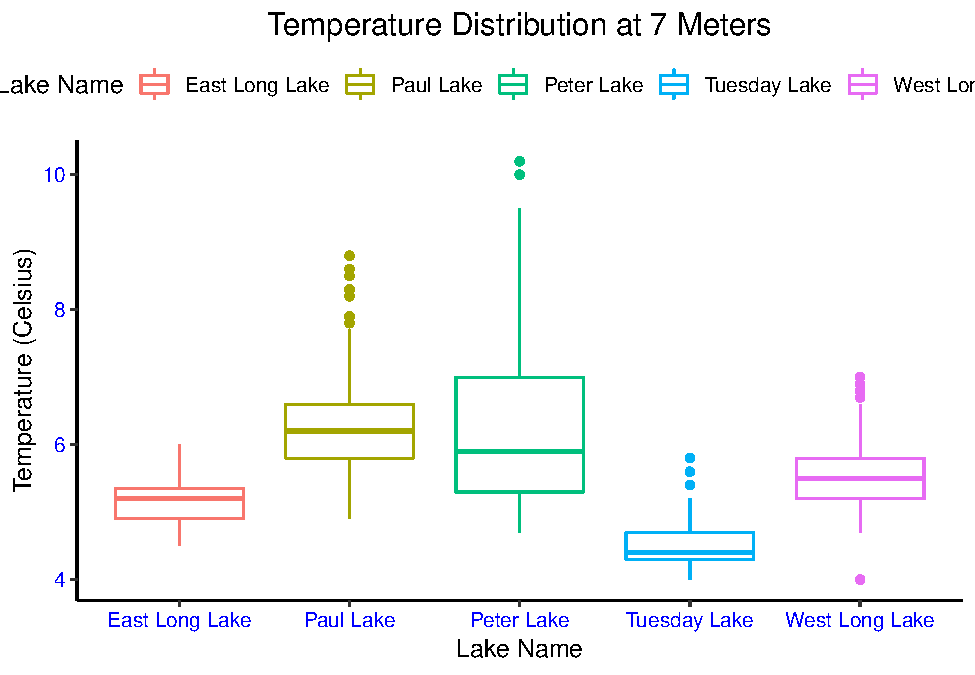
\includegraphics{Bollt_ENV872_FinalProject_files/figure-latex/visualization-1.pdf}

See in the figure titled ``Temperature versus Dissolved Oxygen'' there
is no real correlation between temperature and dissolved oxygen at 7
meters depth across the five lakes.
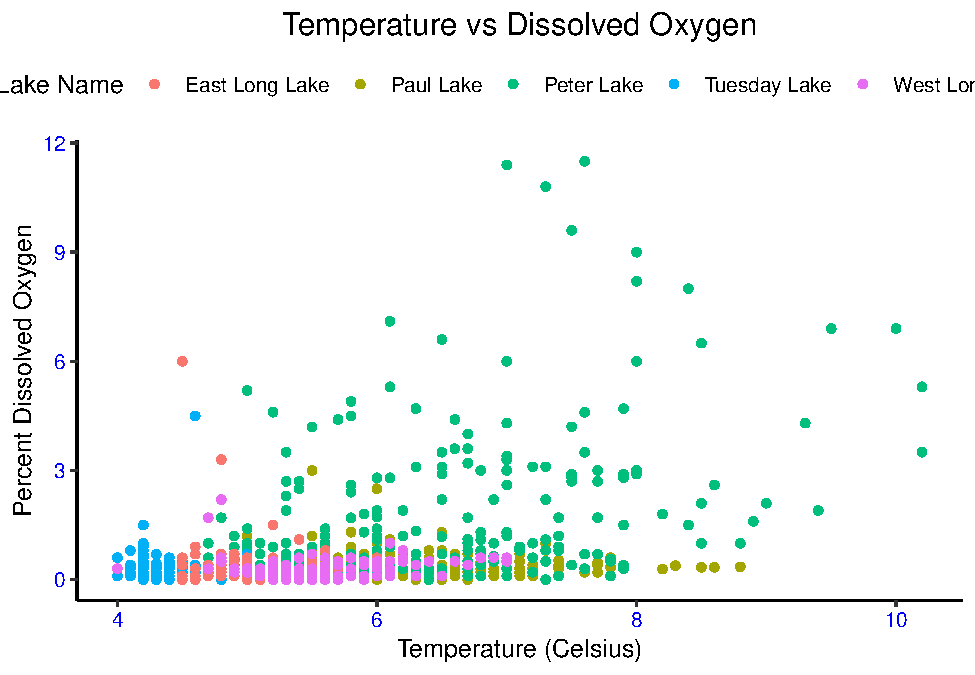
\includegraphics{Bollt_ENV872_FinalProject_files/figure-latex/visualization2-1.pdf}

See in the figure titled ``Paul Lake Temperature Over Time'' there is
not really much of a trend in temperature in Paul Lake at 7 m depth over
time.
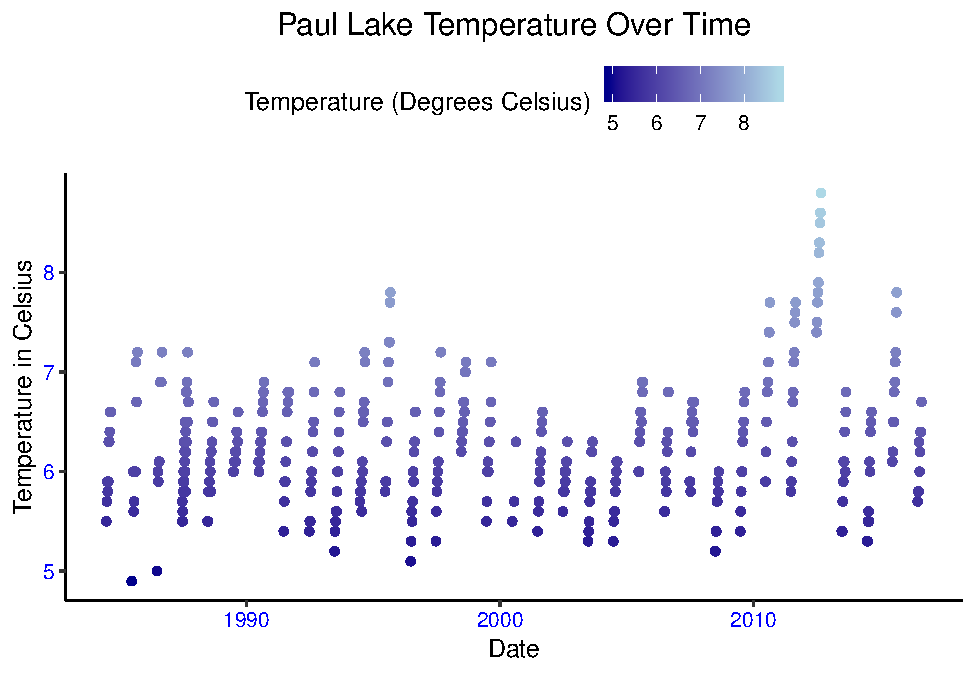
\includegraphics{Bollt_ENV872_FinalProject_files/figure-latex/visualization3-1.pdf}

See in the figure titled ``Paul Lake Dissolved Oxygen Over Time'' there
is not really much of a trend in dissolved oxygen in Paul Lake at 7 m
depth over time.
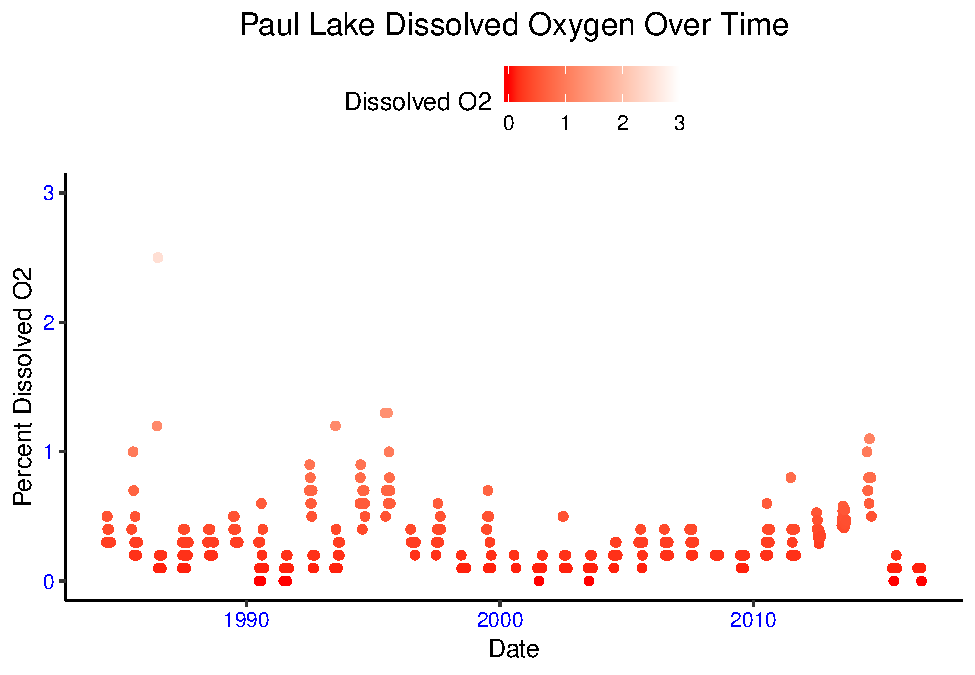
\includegraphics{Bollt_ENV872_FinalProject_files/figure-latex/visualization4-1.pdf}

See in the figure titled ``Paul Lake Temperature Over Time'' that it is
kind of hard to make out a temperature trend in the combined dataset.
This graph has too much data at once and different lakes have different
temporal ranges.
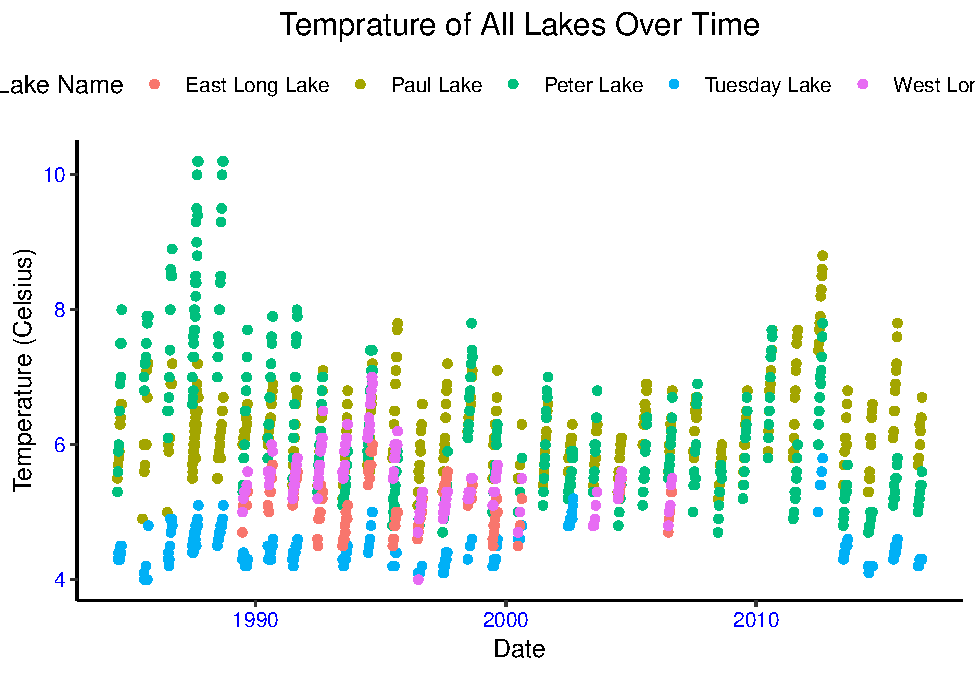
\includegraphics{Bollt_ENV872_FinalProject_files/figure-latex/visualization5-1.pdf}

Overall, my data visualization is not too promising yet. Paul Lake does
not seem to have a trend in either temperature or dissolved oxygen over
time. Likewise, the combined dataset does not appear to have a trend in
temperature over time. However, just because there is not a trend
visible to the naked eye does not mean that a trend does not exist. I
will run a series of statistical analyses on the combined dataset and on
each of the five lakes individually to try and tease out a relationship
that would indicate that thermocline location is moving in response to
climate change.

Analysis:

Now that I have visualized my data, it is time to start running
statistical tests on it in order to answer my research question. I am
interested in two parameters at 7 meters depth, temperature and
dissolved oxygen content. First, I will perform two repeated measures
ANOVAs on the combined processed dataset. I will first run the test on
temperature and then on dissolved oxygen. These two tests takes into
account autocorrelation within a given year and within a given lake.

\begin{Shaded}
\begin{Highlighting}[]
\CommentTok{#Accounting for autocorrelation}
\NormalTok{Alllakestemptest.auto <-}\StringTok{ }\KeywordTok{lme}\NormalTok{(}\DataTypeTok{data =}\NormalTok{ NTL_processed, }
\NormalTok{                     temperature_C }\OperatorTok{~}\StringTok{ }\NormalTok{sampledate }\OperatorTok{*}\StringTok{ }\NormalTok{lakename, }\CommentTok{#fixed effects portion of model: response variable, being predicted based off of sampledate and lakename}
                     \DataTypeTok{random =} \OperatorTok{~}\DecValTok{1}\OperatorTok{|}\NormalTok{Week)  }\CommentTok{# this is the random effect portion of the model}
\NormalTok{Alllakestemptest.auto}
\end{Highlighting}
\end{Shaded}

\begin{verbatim}
## Linear mixed-effects model fit by REML
##   Data: NTL_processed 
##   Log-restricted-likelihood: -1115.039
##   Fixed: temperature_C ~ sampledate * lakename 
##                       (Intercept)                        sampledate 
##                      5.272491e+00                     -2.594702e-06 
##                 lakenamePaul Lake                lakenamePeter Lake 
##                      6.674286e-01                      2.857278e+00 
##              lakenameTuesday Lake            lakenameWest Long Lake 
##                     -7.952465e-01                      1.303065e+00 
##      sampledate:lakenamePaul Lake     sampledate:lakenamePeter Lake 
##                      4.527449e-05                     -1.592099e-04 
##   sampledate:lakenameTuesday Lake sampledate:lakenameWest Long Lake 
##                      1.436851e-05                     -9.102572e-05 
## 
## Random effects:
##  Formula: ~1 | Week
##         (Intercept)  Residual
## StdDev:   0.4782782 0.5869904
## 
## Number of Observations: 1166
## Number of Groups: 14
\end{verbatim}

\begin{Shaded}
\begin{Highlighting}[]
\CommentTok{# we care about the Stddeviation between each week}
\KeywordTok{ACF}\NormalTok{(Alllakestemptest.auto)}
\end{Highlighting}
\end{Shaded}

\begin{verbatim}
##    lag         ACF
## 1    0  1.00000000
## 2    1  0.30030325
## 3    2  0.17631594
## 4    3  0.16396185
## 5    4  0.09572205
## 6    5  0.02603781
## 7    6  0.04758664
## 8    7  0.01355097
## 9    8 -0.03009261
## 10   9 -0.01841401
## 11  10  0.01043748
## 12  11 -0.08491264
## 13  12 -0.02546651
## 14  13 -0.03374768
## 15  14 -0.11342657
## 16  15 -0.09191131
## 17  16 -0.02084283
## 18  17 -0.06995509
## 19  18 -0.14331117
## 20  19 -0.04230610
## 21  20  0.02734688
\end{verbatim}

\begin{Shaded}
\begin{Highlighting}[]
\CommentTok{# we care about the lag of 1's value. This tells us how much temperature is autocorrelated within a given year (it's about 23%)}

\CommentTok{#running the ANOVA}
\NormalTok{Alllakestemptest.mixed <-}\StringTok{ }\KeywordTok{lme}\NormalTok{(}\DataTypeTok{data =}\NormalTok{ NTL_processed,}
\NormalTok{                     temperature_C }\OperatorTok{~}\StringTok{ }\NormalTok{sampledate }\OperatorTok{*}\StringTok{ }\NormalTok{lakename, }
                     \DataTypeTok{random =} \OperatorTok{~}\DecValTok{1}\OperatorTok{|}\NormalTok{Week,}
                     \DataTypeTok{correlation =} \KeywordTok{corAR1}\NormalTok{(}\DataTypeTok{form =} \OperatorTok{~}\StringTok{ }\NormalTok{sampledate}\OperatorTok{/}\NormalTok{lakename}\OperatorTok{|}\NormalTok{Week, }\DataTypeTok{value =} \FloatTok{0.2323}\NormalTok{), }\CommentTok{#correlation from previous model, sampledate/lakename because the model can only do one lake at a time}
                     \DataTypeTok{method =} \StringTok{"REML"}\NormalTok{)}
\end{Highlighting}
\end{Shaded}

\begin{verbatim}
## Warning in eval(aux[[2]], object): Incompatible methods ("Ops.Date",
## "Ops.factor") for "/"

## Warning in eval(aux[[2]], object): Incompatible methods ("Ops.Date",
## "Ops.factor") for "/"

## Warning in eval(aux[[2]], object): Incompatible methods ("Ops.Date",
## "Ops.factor") for "/"

## Warning in eval(aux[[2]], object): Incompatible methods ("Ops.Date",
## "Ops.factor") for "/"

## Warning in eval(aux[[2]], object): Incompatible methods ("Ops.Date",
## "Ops.factor") for "/"

## Warning in eval(aux[[2]], object): Incompatible methods ("Ops.Date",
## "Ops.factor") for "/"

## Warning in eval(aux[[2]], object): Incompatible methods ("Ops.Date",
## "Ops.factor") for "/"

## Warning in eval(aux[[2]], object): Incompatible methods ("Ops.Date",
## "Ops.factor") for "/"

## Warning in eval(aux[[2]], object): Incompatible methods ("Ops.Date",
## "Ops.factor") for "/"

## Warning in eval(aux[[2]], object): Incompatible methods ("Ops.Date",
## "Ops.factor") for "/"

## Warning in eval(aux[[2]], object): Incompatible methods ("Ops.Date",
## "Ops.factor") for "/"

## Warning in eval(aux[[2]], object): Incompatible methods ("Ops.Date",
## "Ops.factor") for "/"

## Warning in eval(aux[[2]], object): Incompatible methods ("Ops.Date",
## "Ops.factor") for "/"

## Warning in eval(aux[[2]], object): Incompatible methods ("Ops.Date",
## "Ops.factor") for "/"
\end{verbatim}

\begin{Shaded}
\begin{Highlighting}[]
\KeywordTok{summary}\NormalTok{(Alllakestemptest.mixed)}
\end{Highlighting}
\end{Shaded}

\begin{verbatim}
## Linear mixed-effects model fit by REML
##  Data: NTL_processed 
##        AIC      BIC    logLik
##   2218.312 2283.998 -1096.156
## 
## Random effects:
##  Formula: ~1 | Week
##         (Intercept)  Residual
## StdDev:   0.4868318 0.5787918
## 
## Correlation Structure: ARMA(1,0)
##  Formula: ~sampledate/lakename | Week 
##  Parameter estimate(s):
##      Phi1 
## 0.6268315 
## Fixed effects: temperature_C ~ sampledate * lakename 
##                                       Value Std.Error   DF   t-value
## (Intercept)                        5.280447 0.3570871 1143 14.787559
## sampledate                        -0.000003 0.0000346 1143 -0.080810
## lakenamePaul Lake                  0.630933 0.3475820 1143  1.815207
## lakenamePeter Lake                 2.697730 0.3474224 1143  7.764987
## lakenameTuesday Lake              -0.835473 0.3526892 1143 -2.368865
## lakenameWest Long Lake             1.338440 0.4495996 1143  2.976961
## sampledate:lakenamePaul Lake       0.000048 0.0000358 1143  1.339615
## sampledate:lakenamePeter Lake     -0.000147 0.0000358 1143 -4.124955
## sampledate:lakenameTuesday Lake    0.000017 0.0000363 1143  0.470521
## sampledate:lakenameWest Long Lake -0.000095 0.0000465 1143 -2.040667
##                                   p-value
## (Intercept)                        0.0000
## sampledate                         0.9356
## lakenamePaul Lake                  0.0698
## lakenamePeter Lake                 0.0000
## lakenameTuesday Lake               0.0180
## lakenameWest Long Lake             0.0030
## sampledate:lakenamePaul Lake       0.1806
## sampledate:lakenamePeter Lake      0.0000
## sampledate:lakenameTuesday Lake    0.6381
## sampledate:lakenameWest Long Lake  0.0415
##  Correlation: 
##                                   (Intr) smpldt lknmPlL lknmPtL lknmTL
## sampledate                        -0.918                              
## lakenamePaul Lake                 -0.889  0.943                       
## lakenamePeter Lake                -0.889  0.943  0.912                
## lakenameTuesday Lake              -0.875  0.929  0.898   0.899        
## lakenameWest Long Lake            -0.683  0.726  0.701   0.702   0.692
## sampledate:lakenamePaul Lake       0.890 -0.968 -0.984  -0.913  -0.900
## sampledate:lakenamePeter Lake      0.889 -0.967 -0.913  -0.984  -0.899
## sampledate:lakenameTuesday Lake    0.876 -0.952 -0.899  -0.899  -0.982
## sampledate:lakenameWest Long Lake  0.681 -0.741 -0.699  -0.699  -0.690
##                                   lknWLL smpldt:lknmPlL smpldt:lknmPtL
## sampledate                                                            
## lakenamePaul Lake                                                     
## lakenamePeter Lake                                                    
## lakenameTuesday Lake                                                  
## lakenameWest Long Lake                                                
## sampledate:lakenamePaul Lake      -0.703                              
## sampledate:lakenamePeter Lake     -0.703  0.937                       
## sampledate:lakenameTuesday Lake   -0.693  0.922          0.922        
## sampledate:lakenameWest Long Lake -0.987  0.718          0.718        
##                                   smp:TL
## sampledate                              
## lakenamePaul Lake                       
## lakenamePeter Lake                      
## lakenameTuesday Lake                    
## lakenameWest Long Lake                  
## sampledate:lakenamePaul Lake            
## sampledate:lakenamePeter Lake           
## sampledate:lakenameTuesday Lake         
## sampledate:lakenameWest Long Lake  0.707
## 
## Standardized Within-Group Residuals:
##         Min          Q1         Med          Q3         Max 
## -2.87087159 -0.54707644 -0.05004423  0.44132449  5.00983807 
## 
## Number of Observations: 1166
## Number of Groups: 14
\end{verbatim}

\begin{Shaded}
\begin{Highlighting}[]
\CommentTok{#There is not a significant trend among all of the lakes at 7m.}
\end{Highlighting}
\end{Shaded}

The results from our mixed effects test demonstrates an important
finding. Observe that the p-value for sampledate is 0.94. This means
that we can reject the null hypothesis that there is a significant
linear correlation between date and temperature of the combined dataset
at 7 meters. This does not supports the idea that the temperature at 7
meters in these lakes as a group is changing.

\begin{Shaded}
\begin{Highlighting}[]
\CommentTok{#oxygen may be autocorrelated with temperature}
\CommentTok{#copy from above, and plug in the oxygen data}
\CommentTok{#Accounting for autocorrelation}
\NormalTok{Alllakesoxygentest.auto <-}\StringTok{ }\KeywordTok{lme}\NormalTok{(}\DataTypeTok{data =}\NormalTok{ NTL_processed, }
\NormalTok{                     dissolvedOxygen }\OperatorTok{~}\StringTok{ }\NormalTok{sampledate }\OperatorTok{*}\StringTok{ }\NormalTok{lakename, }\CommentTok{#fixed effects portion of model: response variable, being predicted based off of sampledate and lakename}
                     \DataTypeTok{random =} \OperatorTok{~}\DecValTok{1}\OperatorTok{|}\NormalTok{Week)  }\CommentTok{# this is the random effect portion of the model}
\NormalTok{Alllakesoxygentest.auto}
\end{Highlighting}
\end{Shaded}

\begin{verbatim}
## Linear mixed-effects model fit by REML
##   Data: NTL_processed 
##   Log-restricted-likelihood: -1818.644
##   Fixed: dissolvedOxygen ~ sampledate * lakename 
##                       (Intercept)                        sampledate 
##                     -2.223387e-01                      5.794808e-05 
##                 lakenamePaul Lake                lakenamePeter Lake 
##                      6.045108e-01                      5.592896e+00 
##              lakenameTuesday Lake            lakenameWest Long Lake 
##                      3.712012e-01                      4.404329e-01 
##      sampledate:lakenamePaul Lake     sampledate:lakenamePeter Lake 
##                     -6.381108e-05                     -4.104614e-04 
##   sampledate:lakenameTuesday Lake sampledate:lakenameWest Long Lake 
##                     -4.852979e-05                     -5.360487e-05 
## 
## Random effects:
##  Formula: ~1 | Week
##         (Intercept) Residual
## StdDev:   0.1085113 1.098537
## 
## Number of Observations: 1166
## Number of Groups: 14
\end{verbatim}

\begin{Shaded}
\begin{Highlighting}[]
\CommentTok{# we care about the Stddeviation between each week}
\KeywordTok{ACF}\NormalTok{(Alllakesoxygentest.auto)}
\end{Highlighting}
\end{Shaded}

\begin{verbatim}
##    lag          ACF
## 1    0  1.000000000
## 2    1  0.064503074
## 3    2  0.287520890
## 4    3  0.152613685
## 5    4 -0.055392421
## 6    5  0.008574120
## 7    6 -0.039858173
## 8    7 -0.146340969
## 9    8 -0.146839546
## 10   9 -0.064558016
## 11  10 -0.135531947
## 12  11 -0.144567507
## 13  12 -0.084667262
## 14  13 -0.104176435
## 15  14 -0.035019680
## 16  15 -0.058042007
## 17  16 -0.041918323
## 18  17 -0.028473480
## 19  18 -0.044312102
## 20  19  0.014538690
## 21  20 -0.002689453
\end{verbatim}

\begin{Shaded}
\begin{Highlighting}[]
\CommentTok{# we care about the lag of 1's value. This tells us how much temperature is autocorrelated within a given year (it's about 6%)}

\CommentTok{#running the ANOVA}
\NormalTok{Alllakesoxygentest.mixed <-}\StringTok{ }\KeywordTok{lme}\NormalTok{(}\DataTypeTok{data =}\NormalTok{ NTL_processed,}
\NormalTok{                     dissolvedOxygen }\OperatorTok{~}\StringTok{ }\NormalTok{sampledate }\OperatorTok{*}\StringTok{ }\NormalTok{lakename, }
                     \DataTypeTok{random =} \OperatorTok{~}\DecValTok{1}\OperatorTok{|}\NormalTok{Week,}
                     \DataTypeTok{correlation =} \KeywordTok{corAR1}\NormalTok{(}\DataTypeTok{form =} \OperatorTok{~}\StringTok{ }\NormalTok{sampledate}\OperatorTok{/}\NormalTok{lakename}\OperatorTok{|}\NormalTok{Week, }\DataTypeTok{value =} \FloatTok{0.0645}\NormalTok{), }\CommentTok{#correlation from previous model, sampledate/lakename because the model can only do one lake at a time}
                     \DataTypeTok{method =} \StringTok{"REML"}\NormalTok{)}
\end{Highlighting}
\end{Shaded}

\begin{verbatim}
## Warning in eval(aux[[2]], object): Incompatible methods ("Ops.Date",
## "Ops.factor") for "/"

## Warning in eval(aux[[2]], object): Incompatible methods ("Ops.Date",
## "Ops.factor") for "/"

## Warning in eval(aux[[2]], object): Incompatible methods ("Ops.Date",
## "Ops.factor") for "/"

## Warning in eval(aux[[2]], object): Incompatible methods ("Ops.Date",
## "Ops.factor") for "/"

## Warning in eval(aux[[2]], object): Incompatible methods ("Ops.Date",
## "Ops.factor") for "/"

## Warning in eval(aux[[2]], object): Incompatible methods ("Ops.Date",
## "Ops.factor") for "/"

## Warning in eval(aux[[2]], object): Incompatible methods ("Ops.Date",
## "Ops.factor") for "/"

## Warning in eval(aux[[2]], object): Incompatible methods ("Ops.Date",
## "Ops.factor") for "/"

## Warning in eval(aux[[2]], object): Incompatible methods ("Ops.Date",
## "Ops.factor") for "/"

## Warning in eval(aux[[2]], object): Incompatible methods ("Ops.Date",
## "Ops.factor") for "/"

## Warning in eval(aux[[2]], object): Incompatible methods ("Ops.Date",
## "Ops.factor") for "/"

## Warning in eval(aux[[2]], object): Incompatible methods ("Ops.Date",
## "Ops.factor") for "/"

## Warning in eval(aux[[2]], object): Incompatible methods ("Ops.Date",
## "Ops.factor") for "/"

## Warning in eval(aux[[2]], object): Incompatible methods ("Ops.Date",
## "Ops.factor") for "/"
\end{verbatim}

\begin{Shaded}
\begin{Highlighting}[]
\KeywordTok{summary}\NormalTok{(Alllakesoxygentest.mixed)}
\end{Highlighting}
\end{Shaded}

\begin{verbatim}
## Linear mixed-effects model fit by REML
##  Data: NTL_processed 
##        AIC      BIC    logLik
##   3913.639 3979.324 -1943.819
## 
## Random effects:
##  Formula: ~1 | Week
##         (Intercept) Residual
## StdDev:   0.1024103 1.225626
## 
## Correlation Structure: ARMA(1,0)
##  Formula: ~sampledate/lakename | Week 
##  Parameter estimate(s):
##       Phi1 
## -0.3060796 
## Fixed effects: dissolvedOxygen ~ sampledate * lakename 
##                                       Value Std.Error   DF   t-value
## (Intercept)                       -0.225185 0.7022547 1143 -0.320660
## sampledate                         0.000058 0.0000732 1143  0.795956
## lakenamePaul Lake                  0.609414 0.7326343 1143  0.831812
## lakenamePeter Lake                 5.783848 0.7333473 1143  7.886915
## lakenameTuesday Lake               0.382413 0.7440595 1143  0.513955
## lakenameWest Long Lake             0.443015 0.9451461 1143  0.468726
## sampledate:lakenamePaul Lake      -0.000064 0.0000755 1143 -0.850561
## sampledate:lakenamePeter Lake     -0.000424 0.0000755 1143 -5.617511
## sampledate:lakenameTuesday Lake   -0.000049 0.0000767 1143 -0.643533
## sampledate:lakenameWest Long Lake -0.000053 0.0000976 1143 -0.543389
##                                   p-value
## (Intercept)                        0.7485
## sampledate                         0.4262
## lakenamePaul Lake                  0.4057
## lakenamePeter Lake                 0.0000
## lakenameTuesday Lake               0.6074
## lakenameWest Long Lake             0.6394
## sampledate:lakenamePaul Lake       0.3952
## sampledate:lakenamePeter Lake      0.0000
## sampledate:lakenameTuesday Lake    0.5200
## sampledate:lakenameWest Long Lake  0.5870
##  Correlation: 
##                                   (Intr) smpldt lknmPlL lknmPtL lknmTL
## sampledate                        -0.987                              
## lakenamePaul Lake                 -0.957  0.946                       
## lakenamePeter Lake                -0.956  0.945  0.916                
## lakenameTuesday Lake              -0.942  0.931  0.903   0.902        
## lakenameWest Long Lake            -0.741  0.732  0.710   0.709   0.699
## sampledate:lakenamePaul Lake       0.957 -0.969 -0.984  -0.916  -0.903
## sampledate:lakenamePeter Lake      0.956 -0.968 -0.916  -0.984  -0.902
## sampledate:lakenameTuesday Lake    0.941 -0.954 -0.902  -0.901  -0.982
## sampledate:lakenameWest Long Lake  0.739 -0.749 -0.709  -0.708  -0.698
##                                   lknWLL smpldt:lknmPlL smpldt:lknmPtL
## sampledate                                                            
## lakenamePaul Lake                                                     
## lakenamePeter Lake                                                    
## lakenameTuesday Lake                                                  
## lakenameWest Long Lake                                                
## sampledate:lakenamePaul Lake      -0.710                              
## sampledate:lakenamePeter Lake     -0.710  0.939                       
## sampledate:lakenameTuesday Lake   -0.699  0.925          0.924        
## sampledate:lakenameWest Long Lake -0.987  0.726          0.726        
##                                   smp:TL
## sampledate                              
## lakenamePaul Lake                       
## lakenamePeter Lake                      
## lakenameTuesday Lake                    
## lakenameWest Long Lake                  
## sampledate:lakenamePaul Lake            
## sampledate:lakenamePeter Lake           
## sampledate:lakenameTuesday Lake         
## sampledate:lakenameWest Long Lake  0.715
## 
## Standardized Within-Group Residuals:
##         Min          Q1         Med          Q3         Max 
## -2.56384702 -0.20032978 -0.06631274  0.10790173  6.81098115 
## 
## Number of Observations: 1166
## Number of Groups: 14
\end{verbatim}

\begin{Shaded}
\begin{Highlighting}[]
\CommentTok{#There is not a significant trend among all of the lakes at 7m.}
\end{Highlighting}
\end{Shaded}

The results from our mixed effects test demonstrates an important
finding. Observe that the p-value for sampledate is 0.43. This means
that we can reject the null hypothesis that there is a significant
linear correlation between date and dissolved oxygen content of combined
dataset at 7 meters. This does not supports the idea that the dissolved
oxygen at 7 meters in these lakes as a group is changing.

While we have rejected the null hypothesis that there is a significant
linear trend between the five lakes for either temperature or dissolved
oxygen, we can still look at trends in the individual lakes. In order to
do this, a seasonal Mann-Kendall test is appropriate. I will run 10
seasonal Mann Kendall tests (five lakes and two parameters per lake). I
will set each year's summer as its own season.

\begin{Shaded}
\begin{Highlighting}[]
\CommentTok{#Paul Lake}
\KeywordTok{length}\NormalTok{(}\KeywordTok{unique}\NormalTok{(Paullake_processed}\OperatorTok{$}\NormalTok{year4)) }\CommentTok{#Tells me how many summers are in the dataset.}
\end{Highlighting}
\end{Shaded}

\begin{verbatim}
## [1] 33
\end{verbatim}

\begin{Shaded}
\begin{Highlighting}[]
\NormalTok{Paullaketemp_ts <-}\StringTok{ }\KeywordTok{ts}\NormalTok{(Paullake_processed}\OperatorTok{$}\NormalTok{temperature_C,}
                      \DataTypeTok{start =} \KeywordTok{c}\NormalTok{(}\DecValTok{1984}\NormalTok{), }\DataTypeTok{frequency =} \DecValTok{33}\NormalTok{)}
\NormalTok{Paullaketemp_ts}
\end{Highlighting}
\end{Shaded}

\begin{verbatim}
## Time Series:
## Start = c(1984, 1) 
## End = c(1994, 25) 
## Frequency = 33 
##   [1] 5.5 5.7 5.9 5.8 5.9 6.3 6.3 6.4 6.6 6.6 4.9 6.0 5.6 5.7 6.0 6.0 6.0
##  [18] 7.1 6.7 7.2 5.0 6.0 5.9 6.1 6.1 6.9 6.9 6.9 7.2 5.5 5.7 5.5 5.6 5.8
##  [35] 5.9 5.8 6.0 5.9 6.3 6.1 6.2 6.0 6.5 5.8 6.4 6.2 6.8 6.3 6.8 6.5 6.9
##  [52] 6.5 7.2 6.7 5.5 5.5 5.8 5.8 5.9 6.1 6.0 5.8 6.2 6.3 6.5 6.5 6.7 6.0
##  [69] 6.0 6.1 6.1 6.2 6.1 6.2 6.4 6.4 6.3 6.6 6.1 6.0 6.1 6.2 6.3 6.3 6.4
##  [86] 6.4 6.6 6.7 6.8 6.9 5.4 5.7 5.9 5.9 6.1 6.3 6.3 6.6 6.8 6.7 6.8 5.4
## [103] 5.5 5.5 5.8 5.9 6.0 6.2 6.2 6.4 6.5 6.8 7.1 5.2 5.4 5.5 5.6 5.6 5.8
## [120] 6.0 6.0 6.2 6.4 6.6 6.8 5.7 5.8 5.8 5.9 5.6 6.1 6.0 6.5 6.6 6.6 6.7
## [137] 7.2 7.1 5.8 5.9 5.9 6.3 6.5 6.5 6.9 7.1 7.3 7.3 7.7 7.8 5.1 5.3 5.6
## [154] 5.5 5.7 6.0 5.9 6.2 6.3 6.6 6.6 5.3 5.6 5.8 5.9 6.0 6.1 6.4 6.6 6.8
## [171] 6.9 7.2 6.2 6.3 6.4 6.4 6.5 6.7 6.7 6.6 7.0 7.0 7.1 5.5 5.7 6.0 6.1
## [188] 6.0 6.3 6.3 6.5 6.5 6.7 7.1 5.5 5.7 6.3 5.4 5.6 5.7 5.9 6.0 6.1 6.2
## [205] 6.4 6.5 6.6 5.6 5.8 5.8 5.8 6.0 5.9 6.0 6.1 6.1 6.3 5.3 5.4 5.5 5.7
## [222] 5.8 5.9 5.8 6.2 6.2 6.3 5.3 5.5 5.6 5.6 5.8 5.9 6.0 6.1 6.1 6.0 6.0
## [239] 6.3 6.4 6.6 6.6 6.5 6.9 6.8 6.9 5.6 5.6 6.0 5.9 5.8 6.3 6.2 6.4 6.8
## [256] 6.8 5.9 5.9 5.8 6.2 6.5 6.6 6.7 6.4 6.5 6.7 5.2 5.2 5.4 5.4 5.7 5.7
## [273] 5.9 5.8 6.0 5.4 5.6 5.8 6.0 6.0 6.3 6.4 6.5 6.7 6.8 5.9 6.2 6.5 6.8
## [290] 6.8 6.9 7.1 7.4 7.4 7.7 5.8 5.9 6.1 6.3 6.7 6.8 7.1 7.2 7.5 7.6 7.7
## [307] 7.4 7.5 7.7 7.8 7.9 8.2 8.3 8.5 8.6 8.8 5.4 5.4 5.7 5.9 6.1 6.1 6.4
## [324] 6.0 6.6 6.8 5.3 5.3 5.5 5.6 5.5 6.1 6.0 6.4 6.5 6.6 6.1 6.2 6.5 6.5
## [341] 6.8 6.9 7.1 7.2 7.6 7.8 5.7 5.8 5.8 6.3 6.0 6.2 6.4 6.4 6.7
\end{verbatim}

\begin{Shaded}
\begin{Highlighting}[]
\NormalTok{Paul_temp_smk <-}\StringTok{ }\KeywordTok{smk.test}\NormalTok{(Paullaketemp_ts)}
\NormalTok{Paul_temp_smk}
\end{Highlighting}
\end{Shaded}

\begin{verbatim}
## 
##  Seasonal Mann-Kendall trend test (Hirsch-Slack test)
## 
## data:  Paullaketemp_ts
## z = 2.2304, p-value = 0.02572
## alternative hypothesis: true S is not equal to 0
## sample estimates:
##        S     varS 
##  159.000 5018.333
\end{verbatim}

\begin{Shaded}
\begin{Highlighting}[]
\KeywordTok{summary}\NormalTok{(Paul_temp_smk) }\CommentTok{#The seasonal Mann Kendall test for temperature at Paul Lake had an overall z-score of 2.2304, an overall p-value of 0.02572 and an overall S value of 159. This test shows a significant positive temperature trend over time at Paul Lake.}
\end{Highlighting}
\end{Shaded}

\begin{verbatim}
## 
##  Seasonal Mann-Kendall trend test (Hirsch-Slack test)
## 
## data: Paullaketemp_ts
## alternative hypothesis: two.sided
## 
## Statistics for individual seasons
## 
## H0
##                      S  varS    tau      z Pr(>|z|)  
## Season 1:   S = 0   -7 161.0 -0.132 -0.473 0.636309  
## Season 2:   S = 0   12 162.0  0.224  0.864 0.387455  
## Season 3:   S = 0    9 160.3  0.170  0.632 0.527519  
## Season 4:   S = 0   13 163.0  0.241  0.940 0.347262  
## Season 5:   S = 0   11 160.3  0.208  0.790 0.429675  
## Season 6:   S = 0   -1 163.0 -0.019  0.000 1.000000  
## Season 7:   S = 0   -2 161.3 -0.037 -0.079 0.937248  
## Season 8:   S = 0    1 156.3  0.019  0.000 1.000000  
## Season 9:   S = 0    8 162.0  0.150  0.550 0.582339  
## Season 10:   S = 0  -2 162.0 -0.037 -0.079 0.937377  
## Season 11:   S = 0  31 163.0  0.574  2.350 0.018784 *
## Season 12:   S = 0  11 156.3  0.212  0.800 0.423834  
## Season 13:   S = 0  21 163.0  0.389  1.567 0.117227  
## Season 14:   S = 0  16 162.0  0.299  1.179 0.238593  
## Season 15:   S = 0  20 164.0  0.367  1.484 0.137902  
## Season 16:   S = 0  12 161.3  0.224  0.866 0.386476  
## Season 17:   S = 0   2 164.0  0.037  0.078 0.937759  
## Season 18:   S = 0  -8 164.0 -0.147 -0.547 0.584648  
## Season 19:   S = 0  -4 164.0 -0.073 -0.234 0.814783  
## Season 20:   S = 0 -16 162.0 -0.299 -1.179 0.238593  
## Season 21:   S = 0  -1 160.3 -0.019  0.000 1.000000  
## Season 22:   S = 0   4 159.3  0.076  0.238 0.812140  
## Season 23:   S = 0  11 161.0  0.208  0.788 0.430632  
## Season 24:   S = 0   6 162.0  0.112  0.393 0.694440  
## Season 25:   S = 0  22 162.0  0.411  1.650 0.098960 .
## Season 26:   S = 0  -1 123.0 -0.023  0.000 1.000000  
## Season 27:   S = 0  -1 123.0 -0.023  0.000 1.000000  
## Season 28:   S = 0   3 123.0  0.068  0.180 0.856890  
## Season 29:   S = 0  12 124.0  0.270  0.988 0.323236  
## Season 30:   S = 0  -1 120.3 -0.023  0.000 1.000000  
## Season 31:   S = 0  -4 122.0 -0.092 -0.272 0.785924  
## Season 32:   S = 0  -7 123.0 -0.159 -0.541 0.588506  
## Season 33:   S = 0 -11 120.3 -0.256 -0.912 0.361976  
## ---
## Signif. codes:  0 '***' 0.001 '**' 0.01 '*' 0.05 '.' 0.1 ' ' 1
\end{verbatim}

\begin{Shaded}
\begin{Highlighting}[]
\NormalTok{Paullakeo2_ts <-}\StringTok{ }\KeywordTok{ts}\NormalTok{(Paullake_processed}\OperatorTok{$}\NormalTok{dissolvedOxygen,}
                      \DataTypeTok{start =} \KeywordTok{c}\NormalTok{(}\DecValTok{1984}\NormalTok{), }\DataTypeTok{frequency =} \DecValTok{33}\NormalTok{)}
\NormalTok{Paullakeo2_ts}
\end{Highlighting}
\end{Shaded}

\begin{verbatim}
## Time Series:
## Start = c(1984, 1) 
## End = c(1994, 25) 
## Frequency = 33 
##   [1] 0.30 0.50 0.50 0.40 0.40 0.40 0.30 0.30 0.30 0.30 0.40 1.00 0.70 0.20
##  [15] 0.30 0.50 0.30 0.30 0.20 0.30 1.20 2.50 0.10 0.10 0.20 0.20 0.10 0.10
##  [29] 0.20 0.30 0.10 0.30 0.20 0.40 0.10 0.40 0.10 0.20 0.10 0.40 0.20 0.20
##  [43] 0.30 0.20 0.10 0.20 0.20 0.20 0.30 0.20 0.20 0.20 0.30 0.30 0.30 0.30
##  [57] 0.40 0.40 0.20 0.40 0.20 0.20 0.20 0.20 0.20 0.20 0.30 0.50 0.40 0.50
##  [71] 0.40 0.30 0.40 0.30 0.30 0.30 0.30 0.30 0.30 0.00 0.10 0.30 0.10 0.00
##  [85] 0.60 0.20 0.10 0.40 0.10 0.10 0.00 0.10 0.00 0.00 0.10 0.20 0.00 0.20
##  [99] 0.10 0.10 0.10 0.70 0.90 0.80 0.60 0.60 0.50 0.70 0.20 0.10 0.10 0.20
## [113] 0.20 0.10 0.10 1.20 0.40 0.10 0.10 0.10 0.20 0.30 0.30 0.20 0.30 0.60
## [127] 0.80 0.90 0.60 0.60 0.40 0.70 0.70 0.70 0.70 0.70 0.60 0.50 1.30 0.50
## [141] 0.70 0.70 0.70 1.30 0.60 0.70 1.00 0.80 0.70 0.60 0.40 0.30 0.30 0.30
## [155] 0.30 0.30 0.30 0.30 0.30 0.20 0.30 0.20 0.30 0.30 0.40 0.60 0.30 0.30
## [169] 0.40 0.40 0.50 0.40 0.20 0.10 0.10 0.10 0.10 0.10 0.10 0.10 0.10 0.10
## [183] 0.10 0.40 0.40 0.50 0.70 0.10 0.50 0.10 0.30 0.10 0.10 0.20 3.00 0.20
## [197] 0.10 0.10 0.10 0.00 0.10 0.10 0.10 0.10 0.10 0.10 0.20 0.50 0.50 0.10
## [211] 0.20 0.10 0.20 0.20 0.10 0.10 0.10 0.10 0.10 0.00 0.10 0.10 0.20 0.20
## [225] 0.20 0.10 0.10 0.20 0.10 0.20 0.20 0.30 0.30 0.30 0.20 0.20 0.30 0.30
## [239] 0.30 0.30 0.40 0.30 0.30 0.10 0.20 0.30 0.40 0.30 0.20 0.30 0.20 0.30
## [253] 0.20 0.20 0.30 0.20 0.40 0.40 0.30 0.20 0.40 0.40 0.30 0.20 0.30 0.30
## [267] 0.20 0.20 0.20 0.20 0.20 0.20 0.20 0.20 0.20 0.20 0.20 0.10 0.20 0.10
## [281] 0.20 0.10 0.10 0.20 0.20 0.20 0.30 0.30 0.60 0.40 0.20 0.30 0.40 0.30
## [295] 0.40 0.80 0.20 0.40 0.30 0.20 0.40 0.20 0.20 0.40 0.20 0.20 0.53 0.40
## [309] 0.47 0.34 0.40 0.29 0.38 0.34 0.34 0.35 0.43 0.48 0.54 0.58 0.49 0.41
## [323] 0.55 0.44 0.45 0.47 1.00 0.70 0.70 0.80 0.60 1.10 0.80 0.80 0.80 0.50
## [337] 0.10 0.10 0.10 0.00 0.10 0.10 0.10 0.10 0.20 0.10 0.10 0.10 0.10 0.10
## [351] 0.10 0.10 0.10 0.10 0.00
\end{verbatim}

\begin{Shaded}
\begin{Highlighting}[]
\NormalTok{Paul_o2_smk <-}\StringTok{ }\KeywordTok{smk.test}\NormalTok{(Paullakeo2_ts)}
\NormalTok{Paul_o2_smk}
\end{Highlighting}
\end{Shaded}

\begin{verbatim}
## 
##  Seasonal Mann-Kendall trend test (Hirsch-Slack test)
## 
## data:  Paullakeo2_ts
## z = -0.43408, p-value = 0.6642
## alternative hypothesis: true S is not equal to 0
## sample estimates:
##        S     varS 
##  -31.000 4776.333
\end{verbatim}

\begin{Shaded}
\begin{Highlighting}[]
\KeywordTok{summary}\NormalTok{(Paul_o2_smk) }\CommentTok{#The seasonal Mann Kendall test for dissolved oxygen at Paul Lake had an overall z-score of -0.434, an overall p-value of 0.66 and an overall S value of -31. This test shows a nonsignificant negative dissolved oxygen trend over time at Paul Lake.}
\end{Highlighting}
\end{Shaded}

\begin{verbatim}
## 
##  Seasonal Mann-Kendall trend test (Hirsch-Slack test)
## 
## data: Paullakeo2_ts
## alternative hypothesis: two.sided
## 
## Statistics for individual seasons
## 
## H0
##                      S  varS    tau      z Pr(>|z|)  
## Season 1:   S = 0    8 153.3  0.159  0.565 0.571869  
## Season 2:   S = 0    5 154.3  0.098  0.322 0.747467  
## Season 3:   S = 0  -13 161.0 -0.245 -0.946 0.344285  
## Season 4:   S = 0    2 159.3  0.038  0.079 0.936856  
## Season 5:   S = 0   -5 151.7 -0.101 -0.325 0.745333  
## Season 6:   S = 0   -3 158.3 -0.058 -0.159 0.873713  
## Season 7:   S = 0  -15 154.3 -0.295 -1.127 0.259771  
## Season 8:   S = 0  -20 150.7 -0.407 -1.548 0.121645  
## Season 9:   S = 0  -18 150.7 -0.366 -1.385 0.166062  
## Season 10:   S = 0  -5 160.3 -0.094 -0.316 0.752079  
## Season 11:   S = 0  -7 158.3 -0.135 -0.477 0.633482  
## Season 12:   S = 0  -4 147.3 -0.081 -0.247 0.804788  
## Season 13:   S = 0 -18 152.7 -0.358 -1.376 0.168862  
## Season 14:   S = 0  -3 147.7 -0.062 -0.165 0.869271  
## Season 15:   S = 0   3 151.7  0.060  0.162 0.870991  
## Season 16:   S = 0 -14 155.3 -0.272 -1.043 0.296919  
## Season 17:   S = 0  -7 154.3 -0.138 -0.483 0.629116  
## Season 18:   S = 0  -6 155.3 -0.117 -0.401 0.688289  
## Season 19:   S = 0 -11 154.3 -0.216 -0.805 0.420847  
## Season 20:   S = 0  -6 154.0 -0.119 -0.403 0.687013  
## Season 21:   S = 0  -8 152.7 -0.159 -0.567 0.571031  
## Season 22:   S = 0 -19 160.3 -0.359 -1.422 0.155158  
## Season 23:   S = 0   7 139.7  0.151  0.508 0.611666  
## Season 24:   S = 0   5 147.7  0.103  0.329 0.742028  
## Season 25:   S = 0   4 155.3  0.078  0.241 0.809782  
## Season 26:   S = 0  28 116.7  0.677  2.500 0.012429 *
## Season 27:   S = 0  10 122.0  0.230  0.815 0.415174  
## Season 28:   S = 0  16 119.3  0.377  1.373 0.169713  
## Season 29:   S = 0  10 115.3  0.242  0.838 0.402008  
## Season 30:   S = 0  12 115.3  0.290  1.024 0.305707  
## Season 31:   S = 0  20 122.0  0.460  1.720 0.085400 .
## Season 32:   S = 0  13 117.7  0.310  1.106 0.268617  
## Season 33:   S = 0   8 107.3  0.205  0.676 0.499254  
## ---
## Signif. codes:  0 '***' 0.001 '**' 0.01 '*' 0.05 '.' 0.1 ' ' 1
\end{verbatim}

\begin{Shaded}
\begin{Highlighting}[]
\CommentTok{#Peter Lake}
\KeywordTok{length}\NormalTok{(}\KeywordTok{unique}\NormalTok{(Peterlake_processed}\OperatorTok{$}\NormalTok{year4)) }\CommentTok{#Tells me how many summers are in the dataset.}
\end{Highlighting}
\end{Shaded}

\begin{verbatim}
## [1] 33
\end{verbatim}

\begin{Shaded}
\begin{Highlighting}[]
\NormalTok{Peterlaketemp_ts <-}\StringTok{ }\KeywordTok{ts}\NormalTok{(Peterlake_processed}\OperatorTok{$}\NormalTok{temperature_C,}
                      \DataTypeTok{start =} \KeywordTok{c}\NormalTok{(}\DecValTok{1984}\NormalTok{), }\DataTypeTok{frequency =} \DecValTok{33}\NormalTok{)}
\NormalTok{Peterlaketemp_ts}
\end{Highlighting}
\end{Shaded}

\begin{verbatim}
## Time Series:
## Start = c(1984, 1) 
## End = c(1994, 21) 
## Frequency = 33 
##   [1]  5.3  5.6  5.9  6.0  6.5  6.9  7.5  7.0  7.5  8.0  7.0  6.8  7.2  7.2
##  [15]  7.3  7.5  7.9  7.8  7.9  6.5  6.1  6.5  6.7  7.0  7.4  8.0  8.6  8.5
##  [29]  8.5  8.9  7.0  6.6  7.3  6.7  7.6  6.8  7.5  7.3  8.0  7.7  8.0  7.7
##  [43]  8.4  7.9  8.5  8.2  9.3  8.4  9.5  9.0 10.0  8.8 10.2  9.4 10.2  7.0
##  [57]  7.3  7.6  7.5  8.0  8.0  8.4  8.5  9.3  9.5 10.0 10.2 10.2  5.3  5.4
##  [71]  5.8  5.8  6.0  6.5  6.5  6.8  7.0  7.3  7.7  5.8  6.1  6.3  6.3  6.7
##  [85]  6.7  7.0  7.2  7.6  7.5  7.9  7.9  5.5  5.8  6.1  6.3  6.6  7.0  7.0
##  [99]  7.5  7.6  8.0  7.9  5.3  5.5  5.7  5.8  6.0  6.2  6.2  6.2  6.6  6.8
## [113]  7.0  7.0  5.1  5.2  5.2  5.2  5.1  5.3  5.5  5.4  5.7  5.7  5.9  5.9
## [127]  5.9  5.8  6.0  6.1  6.3  6.8  7.4  6.8  7.1  6.9  7.4  7.1  4.8  5.2
## [141]  5.0  4.9  5.1  5.3  5.4  5.9  5.6  6.0  5.9  5.8  4.7  4.8  4.9  4.8
## [155]  4.9  5.1  5.0  5.0  5.1  5.3  5.2  4.7  4.9  4.9  5.1  5.1  5.2  5.1
## [169]  5.2  5.3  5.4  5.9  6.1  6.2  6.3  6.7  6.5  6.8  7.0  7.2  7.8  7.4
## [183]  7.3  5.0  5.1  5.3  5.3  5.5  5.6  5.7  6.1  6.0  6.2  6.3  5.0  5.3
## [197]  5.8  5.1  5.3  5.5  5.7  5.8  6.0  6.5  6.4  6.8  6.7  7.0  5.2  5.3
## [211]  5.3  5.4  5.4  5.5  5.4  5.9  5.6  5.8  5.8  5.9  5.3  5.3  5.5  5.6
## [225]  6.0  5.9  6.0  6.4  6.4  6.8  4.8  5.0  5.2  5.4  5.1  5.3  5.5  5.5
## [239]  5.6  5.9  6.0  6.4  6.3  6.4  5.5  5.6  5.7  5.7  5.8  6.0  6.1  6.2
## [253]  6.4  6.7  5.0  5.4  5.6  5.4  5.9  5.5  6.0  6.6  6.7  6.9  4.7  4.9
## [267]  5.1  5.3  5.3  5.6  5.7  5.6  5.5  5.2  5.4  5.4  5.6  5.8  6.1  6.2
## [281]  6.3  6.7  6.5  5.8  6.1  6.3  6.5  6.7  7.0  7.3  7.4  7.7  7.6  4.9
## [295]  5.0  5.3  5.2  5.3  5.5  5.6  5.8  6.0  6.0  6.3  6.5  6.7  7.0  6.9
## [309]  7.1  7.3  7.6  7.8  4.8  4.9  5.0  5.2  5.3  5.3  5.4  5.3  5.4  5.7
## [323]  4.7  4.7  4.8  4.8  4.8  5.0  4.9  5.0  5.0  5.0  5.1  5.2  5.4  5.2
## [337]  5.3  5.5  5.5  5.5  5.7  5.8  5.0  5.1  5.2  5.2  5.3  5.4  5.4  5.4
## [351]  5.6
\end{verbatim}

\begin{Shaded}
\begin{Highlighting}[]
\NormalTok{Peter_temp_smk <-}\StringTok{ }\KeywordTok{smk.test}\NormalTok{(Peterlaketemp_ts)}
\NormalTok{Peter_temp_smk}
\end{Highlighting}
\end{Shaded}

\begin{verbatim}
## 
##  Seasonal Mann-Kendall trend test (Hirsch-Slack test)
## 
## data:  Peterlaketemp_ts
## z = -9.637, p-value < 2.2e-16
## alternative hypothesis: true S is not equal to 0
## sample estimates:
##    S varS 
## -676 4906
\end{verbatim}

\begin{Shaded}
\begin{Highlighting}[]
\KeywordTok{summary}\NormalTok{(Peter_temp_smk) }\CommentTok{#The seasonal Mann Kendall test for temperature at Peter Lake had an overall z-score of -9.637, an overall p-value of <2.2x10^-16 and an overall S value of -676. This test shows a significant negative temperature trend over time at Peter Lake.}
\end{Highlighting}
\end{Shaded}

\begin{verbatim}
## 
##  Seasonal Mann-Kendall trend test (Hirsch-Slack test)
## 
## data: Peterlaketemp_ts
## alternative hypothesis: two.sided
## 
## Statistics for individual seasons
## 
## H0
##                      S  varS    tau      z Pr(>|z|)  
## Season 1:   S = 0  -27 160.3 -0.510 -2.053 0.040039 *
## Season 2:   S = 0  -31 163.0 -0.574 -2.350 0.018784 *
## Season 3:   S = 0  -22 161.3 -0.411 -1.653 0.098266 .
## Season 4:   S = 0  -22 162.0 -0.411 -1.650 0.098960 .
## Season 5:   S = 0  -19 160.3 -0.359 -1.422 0.155158  
## Season 6:   S = 0  -25 165.0 -0.455 -1.868 0.061707 .
## Season 7:   S = 0  -21 165.0 -0.382 -1.557 0.119471  
## Season 8:   S = 0  -23 163.0 -0.426 -1.723 0.084857 .
## Season 9:   S = 0  -22 162.0 -0.411 -1.650 0.098960 .
## Season 10:   S = 0 -20 164.0 -0.367 -1.484 0.137902  
## Season 11:   S = 0 -18 164.0 -0.330 -1.327 0.184351  
## Season 12:   S = 0 -20 164.0 -0.367 -1.484 0.137902  
## Season 13:   S = 0 -26 164.0 -0.477 -1.952 0.050918 .
## Season 14:   S = 0 -21 163.0 -0.389 -1.567 0.117227  
## Season 15:   S = 0 -19 163.0 -0.352 -1.410 0.158578  
## Season 16:   S = 0 -25 165.0 -0.455 -1.868 0.061707 .
## Season 17:   S = 0 -26 164.0 -0.477 -1.952 0.050918 .
## Season 18:   S = 0 -25 163.0 -0.463 -1.880 0.060132 .
## Season 19:   S = 0 -14 164.0 -0.257 -1.015 0.310044  
## Season 20:   S = 0 -13 163.0 -0.241 -0.940 0.347262  
## Season 21:   S = 0 -11 160.3 -0.208 -0.790 0.429675  
## Season 22:   S = 0 -13 125.0 -0.289 -1.073 0.283131  
## Season 23:   S = 0 -13 123.0 -0.296 -1.082 0.279251  
## Season 24:   S = 0 -19 125.0 -0.422 -1.610 0.107405  
## Season 25:   S = 0 -14 121.3 -0.322 -1.180 0.237923  
## Season 26:   S = 0 -16 124.0 -0.360 -1.347 0.177967  
## Season 27:   S = 0 -16 124.0 -0.360 -1.347 0.177967  
## Season 28:   S = 0 -20 121.3 -0.460 -1.725 0.084546 .
## Season 29:   S = 0 -22 124.0 -0.494 -1.886 0.059314 .
## Season 30:   S = 0 -28 124.0 -0.629 -2.425 0.015322 *
## Season 31:   S = 0 -21 123.0 -0.477 -1.803 0.071335 .
## Season 32:   S = 0 -20 124.0 -0.449 -1.706 0.087961 .
## Season 33:   S = 0 -24 124.0 -0.539 -2.065 0.038879 *
## ---
## Signif. codes:  0 '***' 0.001 '**' 0.01 '*' 0.05 '.' 0.1 ' ' 1
\end{verbatim}

\begin{Shaded}
\begin{Highlighting}[]
\NormalTok{Peterlakeo2_ts <-}\StringTok{ }\KeywordTok{ts}\NormalTok{(Peterlake_processed}\OperatorTok{$}\NormalTok{dissolvedOxygen,}
                      \DataTypeTok{start =} \KeywordTok{c}\NormalTok{(}\DecValTok{1984}\NormalTok{), }\DataTypeTok{frequency =} \DecValTok{33}\NormalTok{)}
\NormalTok{Peterlakeo2_ts}
\end{Highlighting}
\end{Shaded}

\begin{verbatim}
## Time Series:
## Start = c(1984, 1) 
## End = c(1994, 21) 
## Frequency = 33 
##   [1]  1.90  1.40  1.80  1.40  2.20  2.20  2.90  2.60  2.80  3.00  1.30
##  [12]  1.10  0.60  1.00  0.50  0.40  0.40  0.50  0.30  6.60  7.10  3.10
##  [23]  3.20  3.00  1.70  2.90  2.60  2.10  1.00  1.60 11.40  3.60 10.80
##  [34]  1.70 11.50  1.30  9.60  2.20  9.00  2.70  8.20  1.70  8.00  1.50
##  [45]  6.50  1.80  4.30  1.50  6.90  2.10  6.90  1.00  5.30  1.90  3.50
##  [56] 11.40 10.80 11.50  9.60  9.00  8.20  8.00  6.50  4.30  6.90  6.90
##  [67]  5.30  3.50  2.70  2.50  2.40  2.60  2.80  3.50  2.90  3.00  3.40
##  [78]  3.10  3.00  2.40  2.80  3.10  3.10  4.00  3.60  3.30  3.10  3.50
##  [89]  2.70  2.80  2.90  4.20  4.90  5.30  4.70  4.40  6.00  4.30  4.20
## [100]  4.60  6.00  4.70  3.50  4.20  4.40  4.50  1.90  1.90  1.20  0.30
## [111]  0.50  0.40  0.50  0.60  0.40  0.10  0.90  0.50  0.40  0.20  0.30
## [122]  0.30  0.40  0.40  0.40  0.40  0.50  1.70  1.20  0.90  0.70  0.70
## [133]  0.90  0.80  0.90  1.00  1.20  0.80  1.70  4.60  1.40  1.20  1.00
## [144]  2.30  1.10  1.30  0.90  1.10  0.60  0.70  0.40  0.40  0.40  0.30
## [155]  0.30  0.30  0.30  0.30  0.30  0.20  0.30  0.20  0.30  0.30  0.70
## [166]  0.30  0.20  0.20  0.40  0.40  0.30  0.30  0.20  0.30  0.20  0.50
## [177]  0.30  0.10  0.10  0.20  0.10  0.10  0.00  0.50  0.40  0.20  0.20
## [188]  0.20  0.20  0.20  0.20  0.20  0.30  0.30  5.20  1.00  0.20  0.10
## [199]  0.10  0.10  0.20  0.30  0.10  0.20  0.00  0.10  0.10  0.30  0.30
## [210]  0.70  0.20  0.10  0.20  0.20  0.20  0.10  0.10  0.10  0.20  0.20
## [221]  0.10  0.10  0.30  0.20  0.10  0.30  0.40  0.20  0.30  0.80  0.20
## [232]  0.20  0.30  0.50  0.30  0.30  0.20  0.30  0.20  0.20  0.30  0.30
## [243]  0.20  0.30  0.30  0.30  0.20  0.30  0.30  0.40  0.40  0.30  0.30
## [254]  0.30  1.00  2.70  1.20  0.70  0.60  0.90  0.80  0.60  0.30  0.50
## [265]  0.20  0.30  0.20  0.20  0.20  0.30  0.30  0.30  0.20  0.30  0.40
## [276]  0.60  1.00  0.40  0.90  0.80  0.70  0.80  0.70  0.30  0.30  0.50
## [287]  0.70  1.00  1.30  1.10  0.80  0.70  0.30  0.20  0.20  0.20  0.20
## [298]  0.10  0.20  0.30  0.40  0.50  1.72  1.34  1.18  1.11  1.20  0.64
## [309]  0.85  0.81  0.70  0.56  0.52  0.56  0.55  0.43  0.52  0.49  0.52
## [320]  0.56  0.52  0.44  1.00  0.60  0.70  0.70  0.70  0.80  0.90  0.80
## [331]  0.90  0.40  0.10  0.10  0.30  0.10  0.10  0.10  0.20  0.00  0.10
## [342]  0.10  0.20  0.10  0.10  0.10  0.00  0.10  0.10  0.10  0.10
\end{verbatim}

\begin{Shaded}
\begin{Highlighting}[]
\NormalTok{Peter_o2_smk <-}\StringTok{ }\KeywordTok{smk.test}\NormalTok{(Peterlakeo2_ts)}
\NormalTok{Peter_o2_smk}
\end{Highlighting}
\end{Shaded}

\begin{verbatim}
## 
##  Seasonal Mann-Kendall trend test (Hirsch-Slack test)
## 
## data:  Peterlakeo2_ts
## z = -10.557, p-value < 2.2e-16
## alternative hypothesis: true S is not equal to 0
## sample estimates:
##        S     varS 
## -738.000 4873.333
\end{verbatim}

\begin{Shaded}
\begin{Highlighting}[]
\KeywordTok{summary}\NormalTok{(Peter_o2_smk) }\CommentTok{#The seasonal Mann Kendall test for dissolved oxygen at Peter Lake had an overall z-score of -10.557, an overall p-value of <2.2x10^-16 and an overall S value of -738. This test shows a significant negative dissolved oxygen trend over time at Peter Lake.}
\end{Highlighting}
\end{Shaded}

\begin{verbatim}
## 
##  Seasonal Mann-Kendall trend test (Hirsch-Slack test)
## 
## data: Peterlakeo2_ts
## alternative hypothesis: two.sided
## 
## Statistics for individual seasons
## 
## H0
##                      S  varS    tau      z  Pr(>|z|)   
## Season 1:   S = 0  -30 162.0 -0.561 -2.278 0.0226995  *
## Season 2:   S = 0  -25 163.0 -0.463 -1.880 0.0601319  .
## Season 3:   S = 0  -32 161.3 -0.598 -2.441 0.0146622  *
## Season 4:   S = 0  -39 163.0 -0.722 -2.976 0.0029166 **
## Season 5:   S = 0  -27 163.0 -0.500 -2.036 0.0417025  *
## Season 6:   S = 0  -31 163.0 -0.574 -2.350 0.0187844  *
## Season 7:   S = 0  -30 161.3 -0.561 -2.283 0.0224211  *
## Season 8:   S = 0  -27 163.0 -0.500 -2.036 0.0417025  *
## Season 9:   S = 0  -32 161.3 -0.598 -2.441 0.0146622  *
## Season 10:   S = 0 -32 156.7 -0.623 -2.477 0.0132603  *
## Season 11:   S = 0 -26 161.3 -0.486 -1.968 0.0490405  *
## Season 12:   S = 0 -27 165.0 -0.491 -2.024 0.0429601  *
## Season 13:   S = 0 -16 164.0 -0.294 -1.171 0.2414769   
## Season 14:   S = 0 -24 161.3 -0.449 -1.811 0.0701749  .
## Season 15:   S = 0 -19 163.0 -0.352 -1.410 0.1585784   
## Season 16:   S = 0 -20 162.0 -0.374 -1.493 0.1354945   
## Season 17:   S = 0 -12 164.0 -0.220 -0.859 0.3903650   
## Season 18:   S = 0 -20 164.0 -0.367 -1.484 0.1379016   
## Season 19:   S = 0 -14 162.0 -0.262 -1.021 0.3070761   
## Season 20:   S = 0 -32 155.3 -0.623 -2.487 0.0128714  *
## Season 21:   S = 0 -23 160.3 -0.434 -1.737 0.0823089  .
## Season 22:   S = 0 -10 119.3 -0.236 -0.824 0.4100103   
## Season 23:   S = 0 -16 121.3 -0.368 -1.362 0.1732730   
## Season 24:   S = 0 -18 124.0 -0.405 -1.527 0.1268493   
## Season 25:   S = 0 -12 124.0 -0.270 -0.988 0.3232363   
## Season 26:   S = 0 -16 124.0 -0.360 -1.347 0.1779674   
## Season 27:   S = 0 -15 125.0 -0.333 -1.252 0.2104977   
## Season 28:   S = 0  -7 123.0 -0.159 -0.541 0.5885064   
## Season 29:   S = 0 -18 121.3 -0.414 -1.543 0.1227507   
## Season 30:   S = 0 -20 121.3 -0.460 -1.725 0.0845458  .
## Season 31:   S = 0 -26 124.0 -0.584 -2.245 0.0247639  *
## Season 32:   S = 0 -19 123.0 -0.432 -1.623 0.1045883   
## Season 33:   S = 0 -23 123.0 -0.523 -1.984 0.0472923  *
## ---
## Signif. codes:  0 '***' 0.001 '**' 0.01 '*' 0.05 '.' 0.1 ' ' 1
\end{verbatim}

\begin{Shaded}
\begin{Highlighting}[]
\CommentTok{#Tuesday Lake}
\KeywordTok{unique}\NormalTok{(Tuesdaylake_processed}\OperatorTok{$}\NormalTok{year4) }\CommentTok{# There are too many gaps in the data, including a 10 year gap from 2002 to 2012 (which is 30% of the length of the timeseries), for me to interpolate the whole dataset for purposes of analysis. I will look at 1984 to 1991, the longest set of continous data collection.}
\end{Highlighting}
\end{Shaded}

\begin{verbatim}
##  [1] 1984 1985 1986 1987 1988 1989 1990 1991 1993 1994 1995 1996 1997 1998
## [15] 1999 2000 2002 2012 2013 2014 2015 2016
\end{verbatim}

\begin{Shaded}
\begin{Highlighting}[]
\NormalTok{Tuesday_smk <-}\StringTok{ }\NormalTok{Tuesdaylake_processed }\OperatorTok
\StringTok{  }\KeywordTok{filter}\NormalTok{(year4 }\OperatorTok{>=}\StringTok{ }\DecValTok{1984}\NormalTok{, year4 }\OperatorTok{<=}\StringTok{ }\DecValTok{1991}\NormalTok{)}
\NormalTok{Tuesdaylaketemp_ts <-}\StringTok{ }\KeywordTok{ts}\NormalTok{(Tuesday_smk}\OperatorTok{$}\NormalTok{temperature_C,}
                      \DataTypeTok{start =} \KeywordTok{c}\NormalTok{(}\DecValTok{1984}\NormalTok{), }\DataTypeTok{frequency =} \DecValTok{8}\NormalTok{)}
\NormalTok{Tuesdaylaketemp_ts}
\end{Highlighting}
\end{Shaded}

\begin{verbatim}
## Time Series:
## Start = c(1984, 1) 
## End = c(1995, 6) 
## Frequency = 8 
##  [1] 4.3 4.4 4.3 4.5 4.4 4.5 4.1 4.0 4.0 4.2 4.0 4.8 4.3 4.4 4.2 4.3 4.5
## [18] 4.9 4.7 4.9 4.9 4.8 4.5 4.4 4.4 4.6 4.4 4.6 4.5 4.7 4.7 4.7 4.5 4.7
## [35] 4.6 4.8 4.7 4.8 4.5 4.8 4.8 4.8 4.8 4.9 4.8 5.1 4.5 4.6 4.6 4.7 4.7
## [52] 4.7 4.8 4.8 4.8 4.8 4.9 5.1 4.3 4.3 4.4 4.3 4.3 4.3 4.2 4.3 4.3 4.2
## [69] 4.2 4.3 4.5 4.3 4.3 4.3 4.3 4.4 4.4 4.3 4.5 4.5 4.5 4.6 4.3 4.4 4.2
## [86] 4.3 4.4 4.4 4.4 4.5 4.5 4.5 4.5 4.6
\end{verbatim}

\begin{Shaded}
\begin{Highlighting}[]
\NormalTok{Tuesday_temp_smk <-}\StringTok{ }\KeywordTok{smk.test}\NormalTok{(Tuesdaylaketemp_ts)}
\NormalTok{Tuesday_temp_smk}
\end{Highlighting}
\end{Shaded}

\begin{verbatim}
## 
##  Seasonal Mann-Kendall trend test (Hirsch-Slack test)
## 
## data:  Tuesdaylaketemp_ts
## z = -0.56165, p-value = 0.5744
## alternative hypothesis: true S is not equal to 0
## sample estimates:
##        S     varS 
##  -23.000 1534.333
\end{verbatim}

\begin{Shaded}
\begin{Highlighting}[]
\KeywordTok{summary}\NormalTok{(Tuesday_temp_smk) }\CommentTok{#The seasonal Mann Kendall test for temperature at Tuesday Lake had an overall z-score of -0.56, an overall p-value of 0.57 and an overall S value of -23. This test shows a nonsignificant negative temperature trend over time at Tuesday Lake.}
\end{Highlighting}
\end{Shaded}

\begin{verbatim}
## 
##  Seasonal Mann-Kendall trend test (Hirsch-Slack test)
## 
## data: Tuesdaylaketemp_ts
## alternative hypothesis: two.sided
## 
## Statistics for individual seasons
## 
## H0
##                     S  varS    tau      z Pr(>|z|)  
## Season 1:   S = 0  11 207.0  0.173  0.695  0.48703  
## Season 2:   S = 0  -1 209.7 -0.016  0.000  1.00000  
## Season 3:   S = 0  -1 195.0 -0.017  0.000  1.00000  
## Season 4:   S = 0 -22 208.7 -0.344 -1.454  0.14601  
## Season 5:   S = 0 -12 206.0 -0.191 -0.766  0.44343  
## Season 6:   S = 0 -15 200.3 -0.245 -0.989  0.32260  
## Season 7:   S = 0   9 148.3  0.181  0.657  0.51127  
## Season 8:   S = 0   8 159.3  0.153  0.555  0.57920  
## ---
## Signif. codes:  0 '***' 0.001 '**' 0.01 '*' 0.05 '.' 0.1 ' ' 1
\end{verbatim}

\begin{Shaded}
\begin{Highlighting}[]
\NormalTok{Tuesdaylakeo2_ts <-}\StringTok{ }\KeywordTok{ts}\NormalTok{(Tuesday_smk}\OperatorTok{$}\NormalTok{dissolvedOxygen,}
                      \DataTypeTok{start =} \KeywordTok{c}\NormalTok{(}\DecValTok{1984}\NormalTok{), }\DataTypeTok{frequency =} \DecValTok{8}\NormalTok{)}
\NormalTok{Tuesdaylakeo2_ts}
\end{Highlighting}
\end{Shaded}

\begin{verbatim}
## Time Series:
## Start = c(1984, 1) 
## End = c(1995, 6) 
## Frequency = 8 
##  [1] 0.3 0.3 0.2 0.3 0.4 0.3 0.2 0.3 0.6 0.2 0.1 0.2 0.1 0.1 0.1 0.1 0.1
## [18] 0.1 0.1 0.1 0.1 0.1 0.2 0.1 0.1 0.3 0.1 0.3 0.1 0.2 0.1 0.1 0.2 0.1
## [35] 0.1 0.0 0.1 0.2 0.1 0.1 0.1 0.1 0.1 0.1 0.2 0.3 0.2 0.3 0.3 0.2 0.1
## [52] 0.1 0.0 0.2 0.1 0.1 0.1 0.3 0.3 0.2 0.2 0.1 0.1 0.2 0.3 0.7 0.2 0.2
## [69] 0.3 0.2 0.2 0.0 0.0 0.0 0.1 0.1 0.4 0.1 0.0 0.2 0.0 0.0 0.0 0.0 0.0
## [86] 0.0 0.0 0.1 0.0 0.0 0.0 0.1 0.1 0.2
\end{verbatim}

\begin{Shaded}
\begin{Highlighting}[]
\NormalTok{Tuesday_o2_smk <-}\StringTok{ }\KeywordTok{smk.test}\NormalTok{(Tuesdaylakeo2_ts)}
\NormalTok{Tuesday_o2_smk}
\end{Highlighting}
\end{Shaded}

\begin{verbatim}
## 
##  Seasonal Mann-Kendall trend test (Hirsch-Slack test)
## 
## data:  Tuesdaylakeo2_ts
## z = -3.3862, p-value = 0.0007088
## alternative hypothesis: true S is not equal to 0
## sample estimates:
##        S     varS 
## -128.000 1406.667
\end{verbatim}

\begin{Shaded}
\begin{Highlighting}[]
\KeywordTok{summary}\NormalTok{(Tuesday_o2_smk) }\CommentTok{#The seasonal Mann Kendall test for dissolved oxygen at Tuesday Lake had an overall z-score of -3.39, an overall p-value of 0.0007 and an overall S value of -128. This test shows a significant negative dissolved oxygen trend over time at Tuesday Lake.}
\end{Highlighting}
\end{Shaded}

\begin{verbatim}
## 
##  Seasonal Mann-Kendall trend test (Hirsch-Slack test)
## 
## data: Tuesdaylakeo2_ts
## alternative hypothesis: two.sided
## 
## Statistics for individual seasons
## 
## H0
##                     S  varS    tau      z Pr(>|z|)  
## Season 1:   S = 0 -30 196.7 -0.503 -2.068 0.038648 *
## Season 2:   S = 0 -20 200.7 -0.329 -1.341 0.179833  
## Season 3:   S = 0 -17 166.3 -0.319 -1.241 0.214755  
## Season 4:   S = 0 -21 190.3 -0.362 -1.450 0.147147  
## Season 5:   S = 0  -1 193.0 -0.017  0.000 1.000000  
## Season 6:   S = 0 -13 186.3 -0.229 -0.879 0.379350  
## Season 7:   S = 0 -20 138.7 -0.437 -1.613 0.106637  
## Season 8:   S = 0  -6 134.7 -0.131 -0.431 0.666567  
## ---
## Signif. codes:  0 '***' 0.001 '**' 0.01 '*' 0.05 '.' 0.1 ' ' 1
\end{verbatim}

\begin{Shaded}
\begin{Highlighting}[]
\CommentTok{#East Long Lake}
\KeywordTok{unique}\NormalTok{(Eastlonglake_processed}\OperatorTok{$}\NormalTok{year4) }\CommentTok{#There are too many gaps in the data, including no data after 2006 (which is 30% of the length of the timeseries), for me to interpolate the whole dataset for purposes of analysis. I will look at 1989 to 2000, the longest set of continous data collection.}
\end{Highlighting}
\end{Shaded}

\begin{verbatim}
##  [1] 1989 1990 1991 1992 1993 1994 1995 1996 1997 1998 1999 2000 2004 2006
\end{verbatim}

\begin{Shaded}
\begin{Highlighting}[]
\NormalTok{Eastlong_smk <-}\StringTok{ }\NormalTok{Eastlonglake_processed }\OperatorTok
\StringTok{  }\KeywordTok{filter}\NormalTok{(year4 }\OperatorTok{>=}\StringTok{ }\DecValTok{1989}\NormalTok{, year4 }\OperatorTok{<=}\StringTok{ }\DecValTok{2000}\NormalTok{)}
\NormalTok{Eastlonglaketemp_ts <-}\StringTok{ }\KeywordTok{ts}\NormalTok{(Eastlong_smk}\OperatorTok{$}\NormalTok{temperature_C,}
                      \DataTypeTok{start =} \KeywordTok{c}\NormalTok{(}\DecValTok{1989}\NormalTok{), }\DataTypeTok{frequency =} \DecValTok{12}\NormalTok{)}
\NormalTok{Eastlonglaketemp_ts}
\end{Highlighting}
\end{Shaded}

\begin{verbatim}
##      Jan Feb Mar Apr May Jun Jul Aug Sep Oct Nov Dec
## 1989 4.7 5.1 5.1 5.1 5.1 5.3 5.1 5.0 5.3 5.3 5.5 5.7
## 1990 5.1 5.3 5.2 5.3 5.5 5.4 5.6 5.6 5.7 5.5 5.6 4.6
## 1991 4.5 4.9 4.9 4.9 5.0 5.0 5.4 5.2 5.2 5.2 5.3 4.5
## 1992 4.5 4.6 4.6 4.6 4.8 4.7 5.0 4.9 4.9 4.9 5.1 5.4
## 1993 5.6 5.7 5.7 5.5 5.7 5.9 5.7 5.9 5.9 6.0 4.5 4.6
## 1994 4.6 4.8 4.8 4.8 4.9 5.0 5.0 5.0 5.0 4.6 4.8 4.7
## 1995 4.8 4.9 4.9 4.9 5.0 5.1 5.0 5.2 5.2 5.3 5.3 5.3
## 1996 5.4 5.4 5.3 5.4 5.5 5.5 5.6 5.6 5.1 5.2 5.2 5.2
## 1997 5.3 5.3 5.3 5.3 5.2 5.4 5.4 4.6 4.5 4.8 4.7 4.8
## 1998 4.9 5.0 5.0 5.2 5.2 5.0 4.5 4.8 5.2
\end{verbatim}

\begin{Shaded}
\begin{Highlighting}[]
\NormalTok{Eastlong_temp_smk <-}\StringTok{ }\KeywordTok{smk.test}\NormalTok{(Eastlonglaketemp_ts)}
\NormalTok{Eastlong_temp_smk}
\end{Highlighting}
\end{Shaded}

\begin{verbatim}
## 
##  Seasonal Mann-Kendall trend test (Hirsch-Slack test)
## 
## data:  Eastlonglaketemp_ts
## z = -0.83753, p-value = 0.4023
## alternative hypothesis: true S is not equal to 0
## sample estimates:
##    S varS 
##  -32 1370
\end{verbatim}

\begin{Shaded}
\begin{Highlighting}[]
\KeywordTok{summary}\NormalTok{(Eastlong_temp_smk) }\CommentTok{#The seasonal Mann Kendall test for temperature at East Long Lake had an overall z-score of -0.84, an overall p-value of 0.40 and an overall S value of -32. This test shows a nonsignificant negative temperature trend over time at East Long Lake.}
\end{Highlighting}
\end{Shaded}

\begin{verbatim}
## 
##  Seasonal Mann-Kendall trend test (Hirsch-Slack test)
## 
## data: Eastlonglaketemp_ts
## alternative hypothesis: two.sided
## 
## Statistics for individual seasons
## 
## H0
##                      S  varS    tau      z Pr(>|z|)  
## Season 1:   S = 0   12 124.0  0.270  0.988 0.323236  
## Season 2:   S = 0    3 123.0  0.068  0.180 0.856890  
## Season 3:   S = 0    5 123.0  0.114  0.361 0.718348  
## Season 4:   S = 0    5 123.0  0.114  0.361 0.718348  
## Season 5:   S = 0    4 122.0  0.092  0.272 0.785924  
## Season 6:   S = 0    1 120.3  0.023  0.000 1.000000  
## Season 7:   S = 0  -10 119.3 -0.236 -0.824 0.410010  
## Season 8:   S = 0  -10 122.0 -0.230 -0.815 0.415174  
## Season 9:   S = 0  -14 121.3 -0.322 -1.180 0.237923  
## Season 10:   S = 0 -12  90.0 -0.343 -1.160 0.246252  
## Season 11:   S = 0 -17  91.0 -0.479 -1.677 0.093492 .
## Season 12:   S = 0   1  91.0  0.028  0.000 1.000000  
## ---
## Signif. codes:  0 '***' 0.001 '**' 0.01 '*' 0.05 '.' 0.1 ' ' 1
\end{verbatim}

\begin{Shaded}
\begin{Highlighting}[]
\NormalTok{Eastlonglakeo2_ts <-}\StringTok{ }\KeywordTok{ts}\NormalTok{(Eastlong_smk}\OperatorTok{$}\NormalTok{dissolvedOxygen,}
                      \DataTypeTok{start =} \KeywordTok{c}\NormalTok{(}\DecValTok{1989}\NormalTok{), }\DataTypeTok{frequency =} \DecValTok{12}\NormalTok{)}
\NormalTok{Eastlonglakeo2_ts}
\end{Highlighting}
\end{Shaded}

\begin{verbatim}
##      Jan Feb Mar Apr May Jun Jul Aug Sep Oct Nov Dec
## 1989 0.4 0.2 0.2 0.2 0.2 0.2 0.3 0.0 0.0 0.3 0.0 0.0
## 1990 0.0 0.0 0.0 0.0 0.0 0.0 0.0 0.2 0.0 0.1 0.1 0.7
## 1991 0.6 0.7 0.6 0.5 0.3 0.3 0.3 0.1 0.1 0.1 0.1 0.1
## 1992 0.0 0.0 0.9 0.1 0.1 0.1 0.1 0.2 0.3 0.3 0.3 1.1
## 1993 0.8 0.4 0.5 0.5 0.3 0.5 0.5 0.4 0.4 0.6 0.6 0.3
## 1994 0.3 0.2 0.4 0.7 0.7 0.6 0.5 0.4 0.3 0.3 0.4 0.1
## 1995 0.3 0.3 0.3 0.2 0.3 0.3 0.3 0.2 0.3 0.3 0.2 0.2
## 1996 0.1 0.2 0.2 0.2 0.4 0.3 0.3 0.3 0.0 0.0 0.1 0.0
## 1997 0.0 0.0 0.0 0.0 0.0 0.0 0.0 0.3 0.4 0.5 0.1 0.1
## 1998 0.1 0.1 0.1 0.1 0.1 0.1 6.0 3.3 0.6
\end{verbatim}

\begin{Shaded}
\begin{Highlighting}[]
\NormalTok{Eastlong_o2_smk <-}\StringTok{ }\KeywordTok{smk.test}\NormalTok{(Eastlonglakeo2_ts)}
\NormalTok{Eastlong_o2_smk}
\end{Highlighting}
\end{Shaded}

\begin{verbatim}
## 
##  Seasonal Mann-Kendall trend test (Hirsch-Slack test)
## 
## data:  Eastlonglakeo2_ts
## z = 0.82562, p-value = 0.409
## alternative hypothesis: true S is not equal to 0
## sample estimates:
##        S     varS 
##   31.000 1320.333
\end{verbatim}

\begin{Shaded}
\begin{Highlighting}[]
\KeywordTok{summary}\NormalTok{(Eastlong_o2_smk) }\CommentTok{#The seasonal Mann Kendall test for dissolved oxygen at East Long Lake had an overall z-score of 0.83, an overall p-value of 0.41 and an overall S value of 31. This test shows a nonsignificant positive dissolved oxygen trend over time at West Long Lake.}
\end{Highlighting}
\end{Shaded}

\begin{verbatim}
## 
##  Seasonal Mann-Kendall trend test (Hirsch-Slack test)
## 
## data: Eastlonglakeo2_ts
## alternative hypothesis: two.sided
## 
## Statistics for individual seasons
## 
## H0
##                      S  varS    tau      z Pr(>|z|)  
## Season 1:   S = 0  -10 119.3 -0.236 -0.824 0.410010  
## Season 2:   S = 0   -7 117.7 -0.167 -0.553 0.580177  
## Season 3:   S = 0  -15 123.0 -0.341 -1.262 0.206827  
## Season 4:   S = 0   -5 118.3 -0.119 -0.368 0.713089  
## Season 5:   S = 0    4 119.3  0.094  0.275 0.783604  
## Season 6:   S = 0    0 119.3  0.000  0.000 1.000000  
## Season 7:   S = 0    9 114.3  0.221  0.748 0.454354  
## Season 8:   S = 0   26 119.3  0.613  2.289 0.022106 *
## Season 9:   S = 0   24 116.7  0.580  2.129 0.033222 *
## Season 10:   S = 0   5  82.3  0.155  0.441 0.659335  
## Season 11:   S = 0   6  83.3  0.183  0.548 0.583882  
## Season 12:   S = 0  -6  87.3 -0.177 -0.535 0.592628  
## ---
## Signif. codes:  0 '***' 0.001 '**' 0.01 '*' 0.05 '.' 0.1 ' ' 1
\end{verbatim}

\begin{Shaded}
\begin{Highlighting}[]
\CommentTok{#West Long Lake}
\KeywordTok{unique}\NormalTok{(Westlonglake_processed}\OperatorTok{$}\NormalTok{year4) }\CommentTok{#There are too many gaps in the data, including no data after 2006 (which is 30% of the length of the timeseries), for me to interpolate the whole dataset for purposes of analysis. I will look at 1989 to 2000, the longest set of continous data collection.}
\end{Highlighting}
\end{Shaded}

\begin{verbatim}
##  [1] 1989 1990 1991 1992 1993 1994 1995 1996 1997 1998 1999 2000 2003 2004
## [15] 2006
\end{verbatim}

\begin{Shaded}
\begin{Highlighting}[]
\NormalTok{Westlong_smk <-}\StringTok{ }\NormalTok{Westlonglake_processed }\OperatorTok
\StringTok{  }\KeywordTok{filter}\NormalTok{(year4 }\OperatorTok{>=}\StringTok{ }\DecValTok{1989}\NormalTok{, year4 }\OperatorTok{<=}\StringTok{ }\DecValTok{2000}\NormalTok{)}
\NormalTok{Westlonglaketemp_ts <-}\StringTok{ }\KeywordTok{ts}\NormalTok{(Westlong_smk}\OperatorTok{$}\NormalTok{temperature_C,}
                      \DataTypeTok{start =} \KeywordTok{c}\NormalTok{(}\DecValTok{1989}\NormalTok{), }\DataTypeTok{frequency =} \DecValTok{12}\NormalTok{)}
\NormalTok{Westlonglaketemp_ts}
\end{Highlighting}
\end{Shaded}

\begin{verbatim}
##      Jan Feb Mar Apr May Jun Jul Aug Sep Oct Nov Dec
## 1989 5.0 5.2 5.3 5.3 5.4 5.6 5.6 5.4 5.5 5.6 6.0 5.9
## 1990 5.2 5.3 5.4 5.5 5.5 5.4 5.6 5.7 5.7 5.8 5.8 5.2
## 1991 5.4 5.5 5.6 5.7 5.7 5.9 6.0 6.1 6.0 6.1 6.5 5.6
## 1992 5.5 5.5 5.6 5.9 5.7 6.0 6.0 6.1 6.1 6.3 6.3 6.1
## 1993 6.1 6.2 6.4 6.2 6.3 6.6 6.7 6.8 7.0 7.0 6.9 5.5
## 1994 5.5 5.6 5.8 6.0 5.8 5.9 6.0 6.0 6.0 6.2 4.7 4.0
## 1995 4.9 4.9 5.0 5.0 5.1 5.2 5.1 5.3 5.3 4.9 5.0 5.1
## 1996 5.1 5.0 5.1 5.1 5.2 5.3 5.3 5.3 5.2 5.2 5.3 5.2
## 1997 5.3 5.3 5.3 5.5 5.5 5.5 5.5 5.1 5.1 5.3 5.3 5.3
## 1998 5.5 5.5 5.5 5.6 5.7 5.7 4.7 5.0 5.5
\end{verbatim}

\begin{Shaded}
\begin{Highlighting}[]
\NormalTok{Westlong_temp_smk <-}\StringTok{ }\KeywordTok{smk.test}\NormalTok{(Westlonglaketemp_ts)}
\NormalTok{Westlong_temp_smk}
\end{Highlighting}
\end{Shaded}

\begin{verbatim}
## 
##  Seasonal Mann-Kendall trend test (Hirsch-Slack test)
## 
## data:  Westlonglaketemp_ts
## z = -1.646, p-value = 0.09975
## alternative hypothesis: true S is not equal to 0
## sample estimates:
##        S     varS 
##  -62.000 1373.333
\end{verbatim}

\begin{Shaded}
\begin{Highlighting}[]
\KeywordTok{summary}\NormalTok{(Westlong_temp_smk) }\CommentTok{#The seasonal Mann Kendall test for temperature at West Long Lake had an overall z-score of -1.65, an overall p-value of 0.10 and an overall S value of -62. This test shows a nonsignificant negative temperature trend over time at West Long Lake.}
\end{Highlighting}
\end{Shaded}

\begin{verbatim}
## 
##  Seasonal Mann-Kendall trend test (Hirsch-Slack test)
## 
## data: Westlonglaketemp_ts
## alternative hypothesis: two.sided
## 
## Statistics for individual seasons
## 
## H0
##                      S  varS    tau      z Pr(>|z|)  
## Season 1:   S = 0    8 121.3  0.184  0.635 0.525110  
## Season 2:   S = 0    3 120.3  0.070  0.182 0.855331  
## Season 3:   S = 0   -1 123.0 -0.023  0.000 1.000000  
## Season 4:   S = 0    2 124.0  0.045  0.090 0.928444  
## Season 5:   S = 0    3 120.3  0.070  0.182 0.855331  
## Season 6:   S = 0   -4 124.0 -0.090 -0.269 0.787616  
## Season 7:   S = 0  -15 120.3 -0.349 -1.276 0.201868  
## Season 8:   S = 0  -21 123.0 -0.477 -1.803 0.071335 .
## Season 9:   S = 0  -13 123.0 -0.296 -1.082 0.279251  
## Season 10:   S = 0  -4  92.0 -0.111 -0.313 0.754454  
## Season 11:   S = 0  -9  91.0 -0.254 -0.839 0.401678  
## Season 12:   S = 0 -11  91.0 -0.310 -1.048 0.294507  
## ---
## Signif. codes:  0 '***' 0.001 '**' 0.01 '*' 0.05 '.' 0.1 ' ' 1
\end{verbatim}

\begin{Shaded}
\begin{Highlighting}[]
\NormalTok{Westlonglakeo2_ts <-}\StringTok{ }\KeywordTok{ts}\NormalTok{(Westlong_smk}\OperatorTok{$}\NormalTok{dissolvedOxygen,}
                      \DataTypeTok{start =} \KeywordTok{c}\NormalTok{(}\DecValTok{1989}\NormalTok{), }\DataTypeTok{frequency =} \DecValTok{12}\NormalTok{)}
\NormalTok{Westlonglakeo2_ts}
\end{Highlighting}
\end{Shaded}

\begin{verbatim}
##      Jan Feb Mar Apr May Jun Jul Aug Sep Oct Nov Dec
## 1989 0.2 0.2 0.2 0.3 0.2 0.2 0.2 0.3 0.0 0.6 0.1 0.0
## 1990 0.0 0.0 0.0 0.0 0.0 0.0 0.0 0.0 0.1 0.1 0.1 0.5
## 1991 0.6 0.7 0.6 0.4 0.5 0.4 0.3 0.1 0.1 0.1 0.1 0.0
## 1992 0.0 0.1 0.4 0.1 0.1 0.1 0.1 0.2 0.3 0.1 0.4 0.5
## 1993 1.0 0.8 0.5 0.5 0.4 0.5 0.4 0.6 0.6 0.5 0.6 0.3
## 1994 0.2 0.3 0.3 0.5 0.6 0.5 0.3 0.4 0.3 0.6 0.3 0.3
## 1995 0.3 0.3 0.3 0.3 0.3 0.3 0.3 0.3 0.2 0.2 0.2 0.2
## 1996 0.1 0.2 0.1 0.1 0.4 0.4 0.3 0.3 0.1 0.1 0.1 0.1
## 1997 0.0 0.1 0.0 0.0 0.0 0.0 0.0 0.3 0.2 0.4 0.1 0.1
## 1998 0.1 0.1 0.1 0.1 0.1 0.1 1.7 0.2 0.1
\end{verbatim}

\begin{Shaded}
\begin{Highlighting}[]
\NormalTok{Westlong_o2_smk <-}\StringTok{ }\KeywordTok{smk.test}\NormalTok{(Westlonglakeo2_ts)}
\NormalTok{Westlong_o2_smk}
\end{Highlighting}
\end{Shaded}

\begin{verbatim}
## 
##  Seasonal Mann-Kendall trend test (Hirsch-Slack test)
## 
## data:  Westlonglakeo2_ts
## z = -0.46921, p-value = 0.6389
## alternative hypothesis: true S is not equal to 0
## sample estimates:
##        S     varS 
##  -18.000 1312.667
\end{verbatim}

\begin{Shaded}
\begin{Highlighting}[]
\KeywordTok{summary}\NormalTok{(Westlong_o2_smk) }\CommentTok{#The seasonal Mann Kendall test for dissolved oxygen at West Long Lake had an overall z-score of -0.47, an overall p-value of 0.64 and an overall S value of -18. This test shows a nonsignificant negative dissolved oxygen trend over time at West Long Lake.}
\end{Highlighting}
\end{Shaded}

\begin{verbatim}
## 
##  Seasonal Mann-Kendall trend test (Hirsch-Slack test)
## 
## data: Westlonglakeo2_ts
## alternative hypothesis: two.sided
## 
## Statistics for individual seasons
## 
## H0
##                      S  varS    tau      z Pr(>|z|)  
## Season 1:   S = 0   -6 119.3 -0.141 -0.458  0.64716  
## Season 2:   S = 0   -6 119.3 -0.141 -0.458  0.64716  
## Season 3:   S = 0  -14 122.0 -0.322 -1.177  0.23921  
## Season 4:   S = 0   -7 118.3 -0.167 -0.552  0.58125  
## Season 5:   S = 0   -2 122.0 -0.046 -0.091  0.92786  
## Season 6:   S = 0   -1 121.0 -0.023  0.000  1.00000  
## Season 7:   S = 0   12 115.3  0.290  1.024  0.30571  
## Season 8:   S = 0    6 115.3  0.145  0.466  0.64152  
## Season 9:   S = 0    5 114.3  0.123  0.374  0.70834  
## Season 10:   S = 0   1  82.3  0.031  0.000  1.00000  
## Season 11:   S = 0   0  75.3  0.000  0.000  1.00000  
## Season 12:   S = 0  -6  88.0 -0.177 -0.533  0.59403  
## ---
## Signif. codes:  0 '***' 0.001 '**' 0.01 '*' 0.05 '.' 0.1 ' ' 1
\end{verbatim}

My data does not appear to be showing a significant change in the
thermocline of any of the five individual lakes, as defined by both
higher temperatures and lower oxygen levels at 7 meters depth. Let's
visualize the temperature and oxygen over the period of the ten tests I
just ran to see if the naked eye agrees with my statistical analysis.

See in ``Dissolved Oxygen Over Time in Each Lake'' that the seasonal
Mann Kendall results for the five lakes do not show an overall dissolved
oxygen trend at 7 meters in a particular direction.
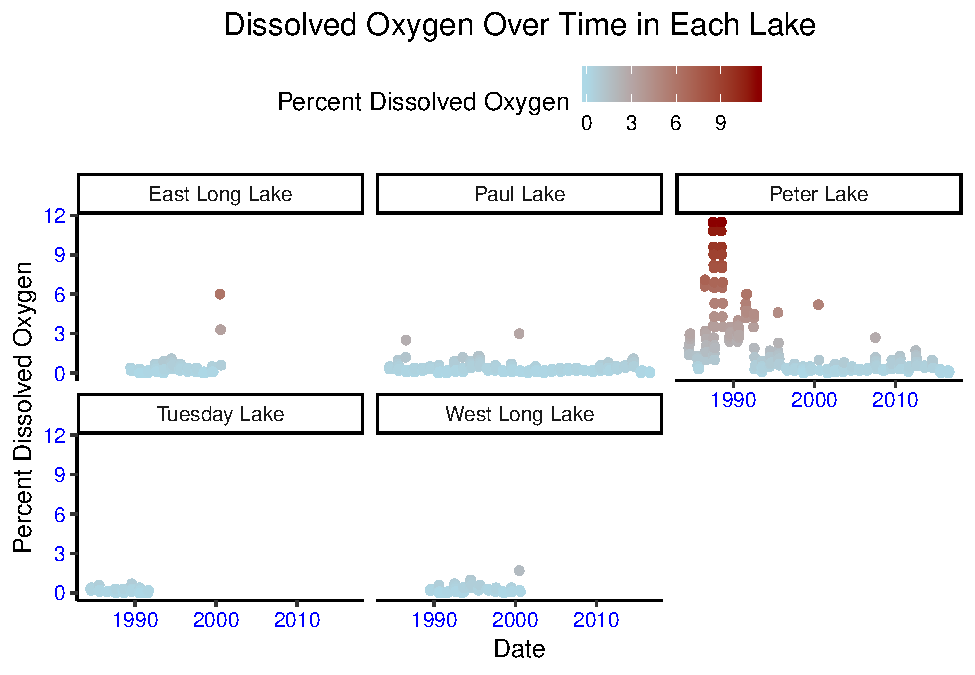
\includegraphics{Bollt_ENV872_FinalProject_files/figure-latex/smk oxygen visualization-1.pdf}

See in ``Temperature Over Time in Each Lake'' that the seasonal Mann
Kendall results for the five lakes do not show an overall temperature
trend at 7 meters in a particular direction.
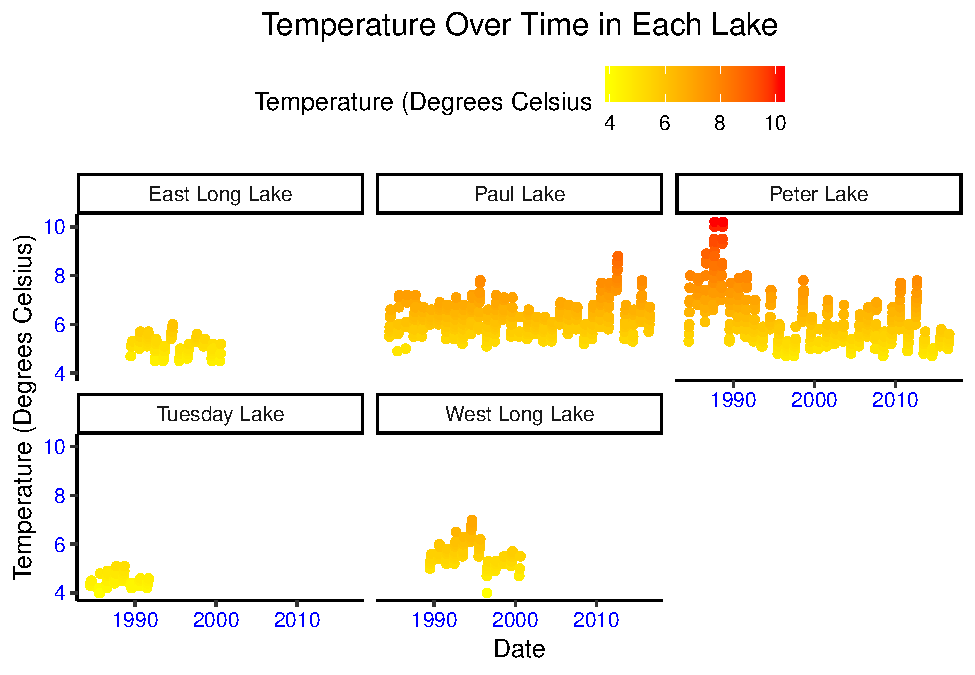
\includegraphics{Bollt_ENV872_FinalProject_files/figure-latex/smk temperature visualization-1.pdf}

Discussion: The results of my tests seem to run contrary to the idea
that climate change is affecting the water temperatures of the lakes in
this study. However, it may be the case that my tests are inconclusive
by design. I am testing whether the thermocline on these lakes is moving
over time. The location of a lake's thermocline is a product of water
chemistry and physics, especially water density. It may be the case that
the basic physics of water that determine where a thermocline sets up
are not affected by 1 °C of global warming. Perhaps, given relatively
modest warming, it is the relative water density that determines where
the thermocline location sets up. It may be the case that the steepness
and not the location of the thermocline is what is changing under
relatively small amounts of warming. If I were to test surface water
temperature or water temperature at, say, 15 meters, I would likely see
evidence of climate change. It might require larger levels of warming
for the thermocline itself to also move. Unfortunately, testing this
hypothesis is beyond the scope of the dataset I am analyzing.


\end{document}
